% (c) 2012 Silvia Cibola - silvia.cibola@gmail.com

% (c) 2012-2014 Dimitrios Vrettos - d.vrettos@gmail.com

\chapter{Vettori}

\section{Prime definizioni}

Sappiamo che due punti~$A$ e~$B$ presi su una retta~$a$ determinano il segmento~$b$ di estremi~$A$ e~$B$; fissiamo su di esso un verso di percorrenza, per esempio da~$A$ verso~$B$.

\begin{definizione}
Il \emph{segmento orientato} di estremi~$A$ e~$B$ si chiama \emph{vettore}; esso viene indicato con~$\overrightarrow{AB}$ oppure con~$\vec{u}$;
il punto~$A$ è il primo estremo e~$B$ il secondo estremo.
\end{definizione}

Un \emph{vettore libero} è caratterizzato da tre elementi:
\begin{itemize*}
\item la \emph{direzione} indicata dalla retta su cui esso giace;
\item il \emph{verso} indicato dalla punta della freccia che dal primo estremo va al secondo estremo;
\item il \emph{modulo} o \emph{intensità}, uguale alla misura del segmento~$AB$: scriveremo~$|\vec{u}|=\overline{AB}$ e leggeremo ``il modulo del vettore~$\vec{u}$ è
uguale alla misura del segmento~$AB$''.
\end{itemize*}

Un \emph{vettore applicato} è caratterizzato, oltre che dai tre elementi suddetti, anche dal \emph{punto di applicazione},
ovvero il punto da cui parte la freccia, chiamato anche primo estremo del vettore.

\begin{exrig}
\begin{esempio}
I due vettori~$\overrightarrow{AB}$ e~$\overrightarrow{DC}$ nella figura~\ref{fig:F.1} appartengono alla stessa retta, quindi hanno stessa direzione, verso opposto e modulo diverso.
\end{esempio}

\begin{esempio}
I due vettori~$\overrightarrow{AB}$ e~$\overrightarrow{DC}$ in figura \ref{fig:F.2} appartengono a rette parallele, quindi hanno stessa direzione. I loro versi sono opposti e hanno
uguale intensità: essi si chiamano \emph{vettori opposti} e scriveremo~$\overrightarrow{AB}=-\overrightarrow{DC}$.
\end{esempio}
\begin{esempio}
I due vettori~$\overrightarrow{AB}$ e~$\overrightarrow{CD}$ in figura \ref{fig:F.3} appartengono a rette parallele, quindi hanno stessa direzione. Hanno lo stesso verso e uguale intensità:
essi si chiamano \emph{equipollenti} e scriveremo~$\overrightarrow{AB}\equiv\overrightarrow{CD}$.
\end{esempio}
\end{exrig}

\begin{figure}[hb]
\centering
% (c) 2012 Dimitrios Vrettos - d.vrettos@gmail.com


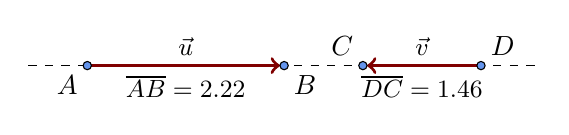
\begin{tikzpicture}[x=5mm,y=5mm]
\begin{scope}[dashed]

\draw (-1,0) -- (12,0);
\end{scope}
\begin{scope}[Maroon, very thick,->, shorten >=1.5pt]
\draw (.5,0) -- (5.5,0);
\draw  (10.5,0)--(7.5,0);
\end{scope}

\node [below left] at (.5,0) {$A$};
\node [below right] at (5.5,0) {$B$};
\node [above left] at (7.5,0) {$C$};
\node [above right] at (10.5,0) {$D$};

\begin{scope}[font=\small]
\node[below] at (9,0) {$\overline{DC}=1.46$};
\node[above] at (9,0) {$\vec{v}$};
\node[below] at (3,0) {$\overline{AB}=2.22$};
\node[above] at (3,0) {$\vec{u}$};
\end{scope}

\foreach \x in {.5,5.5,7.5,10.5}
\filldraw[fill=CornflowerBlue, draw=black] (\x,0) circle (1.5pt);
\end{tikzpicture}
\caption{I vettori hanno stessa direzione, verso opposto e modulo diverso.}\label{fig:F.1}
\end{figure}

 \begin{figure}[ht]
\begin{minipage}{0.45\textwidth}
\centering
\input{./lbr/chapB/fig002_vet.pgf}
\caption{Vettori opposti.}\label{fig:F.2}
\end{minipage}\hfil
\begin{minipage}{0.45\textwidth}
\centering
% (c) 2012 Dimitrios Vrettos - d.vrettos@gmail.com

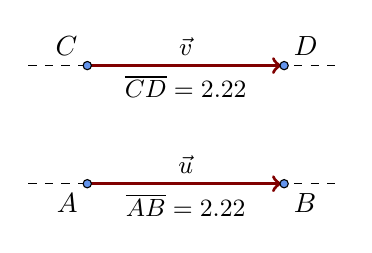
\begin{tikzpicture}[x=5mm,y=5mm]
  \begin{scope}[dashed]
    \foreach \y in {0,3}
      \draw (-1,\y) -- (7,\y);
  \end{scope}
  
  \begin{scope}[Maroon, very thick,->, shorten >=1pt]
    \draw (.5,0) -- (5.5,0);
    \draw (.5,3) -- (5.5,3);
  \end{scope}

  \node [below left] at (.5,0) {$A$};
  \node [below right] at (5.5,0) {$B$};
  \node [above left] at (.5,3) {$C$};
  \node [above right] at (5.5,3) {$D$};

  \begin{scope}[font=\small]
    \node[below] at (3,3) {$\overline{CD}=2.22$};
    \node[above] at (3,3) {$\vec{v}$};
    \node[below] at (3,0) {$\overline{AB}=2.22$};
    \node[above] at (3,0) {$\vec{u}$};
  \end{scope}

  \foreach \x in {.5,5.5}{
    \foreach \yi in {0,3}
      \filldraw[fill=CornflowerBlue, draw=black] (\x,\yi) circle (1.5pt);}
\end{tikzpicture}
\caption{Vettori equipollenti.}\label{fig:F.3}
\end{minipage}
\end{figure}

Osserviamo che un vettore può essere interpretato come uno spostamento dal primo estremo al secondo estremo, avente la direzione della retta cui appartiene il vettore stesso nel
verso indicato dalla freccia.
Nel piano dotato di riferimento cartesiano ortogonale (figura~\ref{fig:F.4} (a)) è rappresentato il vettore~$\vec{u}=\overrightarrow{AB}$ avente il primo estremo nel punto~$A(-2;1)$ e
il secondo estremo
in~$B(1;2)$. Per andare da~$A$ a~$B$ si possono compiere diversi percorsi: possiamo procedere sul vettore~$\vec{u}$ oppure possiamo scegliere di compiere due spostamenti particolari,
uno parallelo all'asse~$x$ e l'altro parallelo all'asse~$y$. In tal modo si determina il punto~$C(1;1)$ come ``tappa intermedia'' per raggiungere~$B$:
ci spostiamo sul vettore~$\overrightarrow{AC}$ e poi da~$C$ sul vettore~$\overrightarrow{CB}$.

\begin{figure}[htb]
\centering
% (c) 2012 Dimitrios Vrettos - d.vrettos@gmail.com

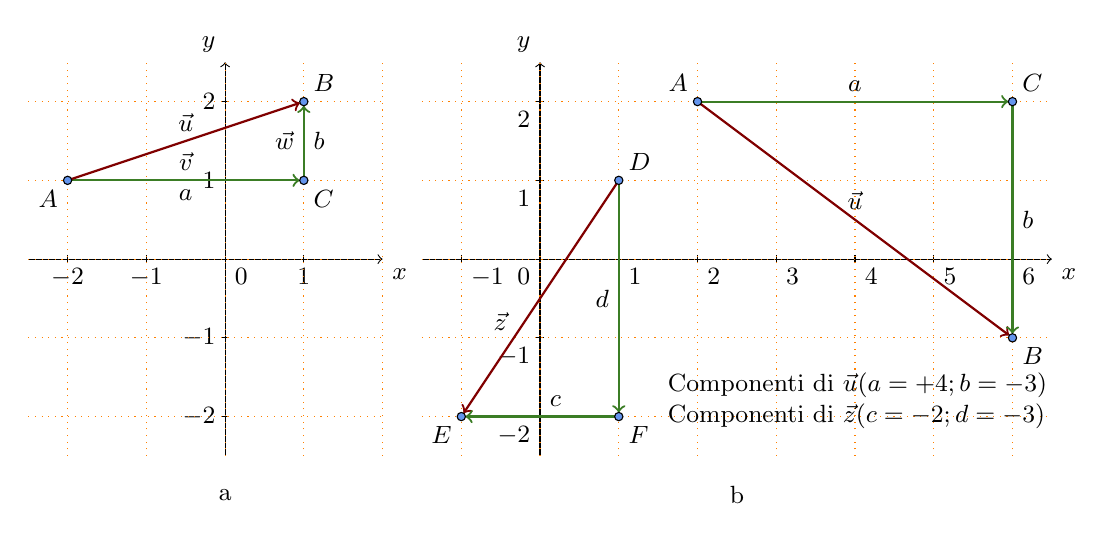
\begin{tikzpicture}[x=10mm,y=10mm, font=\small]

  \begin{scope}[->]
    \draw (-2.5,0) -- (2,0) node [below right] () {$x$};
    \draw (0,-2.5) -- (0,2.5) node[above left] {$y$};
  \end{scope}

  \foreach \x/\xtext in {-2/-2,-1/-1, 1/1}{
    \node[below] at (\x,0) {$\xtext$};
    \draw (\x,1.5pt) -- (\x,-1.5pt);}
  \foreach \y/\ytext in {-2/-2,-1/-1, 1/1, 2/2}{
    \node[left] at (0,\y) {$\ytext$};
    \draw (1.5pt,\y) -- (-1.5pt,\y);}
  \node[below right] at (0,0) {$0$};

  \node[below left] at (-2,1) {$A$};
  \node[above right] at (1,2) {$B$};
  \node[below right] at (1,1) {$C$};

  \node[above] at (-.5,1.5) {$\vec{u}$};
  
  \node[above] at (-.5,1) {$\vec{v}$};
  \node[below] at (-.5,1) {$a$};
  \node[left] at (1,1.5) {$\vec{w}$};
  \node[right] at (1,1.5) {$b$};

\node at (0,-3) {a};
  \begin{scope}[dotted, orange]
    \draw (-2.5,-2.5) grid (2,2.5);
  \end{scope}

  \begin{scope}[thick, OliveGreen, shorten >=1.5pt, ->]
    \draw (-2,1) -- (1,1);
    \draw[Maroon] (-2,1) -- (1,2);
    \draw (1,1) -- (1,2);
  \end{scope}
  
  \begin{scope}[fill=CornflowerBlue, draw=black]
    \filldraw (-2,1) circle (1.5pt);
    \filldraw (1,2) circle (1.5pt);
    \filldraw (1,1) circle (1.5pt);
  \end{scope}

  \begin{scope}[xshift=40mm]
    \begin{scope}[->]
    \draw (-1.5,0) -- (6.5,0) node [below right] () {$x$};
    \draw (0,-2.5) -- (0,2.5) node[above left] {$y$};
    \end{scope}

    \foreach \x/\xtext in {-1/-1, 1/1,2/2,3/3,4/4,5/5,6/6}{
      \node[below right] at (\x,0) {$\xtext$};
      \draw (\x,1.5pt) -- (\x,-1.5pt);}
    \foreach \y/\ytext in {-2/-2,-1/-1, 1/1, 2/2}{
      \node[below left] at (0,\y) {$\ytext$};
      \draw (1.5pt,\y) -- (-1.5pt,\y);}
    \node[below left] at (0,0) {$0$};

    \node[above left] at (2,2) {$A$};
    \node[below right] at (6,-1) {$B$};
    \node[above right] at (6,2) {$C$};

    \node[above] at (4,2) {$a$};
    \node[right] at (6,.5) {$b$};
    \node[above] at (4,.5) {$\vec{u}$};

    \node[above right] at (0,-2) {$c$};
    \node[left] at (1,-.5) {$d$};
    \node[left] at (-.3,-.8) {$\vec{z}$};

    \node[above right] at (1,1) {$D$};
    \node[below right] at (1,-2) {$F$};
    \node[below left] at (-1,-2) {$E$};

    \node at (2.5,-3) {b};
    \begin{scope}[dotted, orange]
      \draw (-1.5,-2.5) grid (6.5,2.5);
    \end{scope}

    \begin{scope}[thick, shorten >=1.5pt, ->]
      \begin{scope}[Maroon]
	\draw(2,2) -- (6,-1);
	\draw (1,1) -- (-1,-2);
      \end{scope}
      
      \begin{scope}[OliveGreen]
	\draw(2,2) -- (6,2);
	\draw (6,2) -- (6,-1);

	\draw (1,1) -- (1,-2);
	\draw (1,-2) -- (-1,-2);
	\end{scope}
    \end{scope}

    \begin{scope}[fill=CornflowerBlue, draw=black]
      \filldraw (6,2) circle (1.5pt);
      \filldraw (2,2) circle (1.5pt);
      \filldraw (6,-1) circle (1.5pt);

      \filldraw (1,1) circle (1.5pt);
      \filldraw (1,-2) circle (1.5pt);
      \filldraw (-1,-2) circle (1.5pt);
    \end{scope}

    \node[right] () at (1.5,-1.6) {Componenti di $\vec{u}(a=+4;b=-3)$};
    \node[right] () at (1.5,-2) {Componenti di $\vec{z}(c=-2;d=-3)$};
  \end{scope}
\end{tikzpicture}
\caption{Spostamenti di vettori.}\label{fig:F.4}
\end{figure}

\begin{definizione}
Chiamiamo \emph{componenti} del vettore~$\overrightarrow{AB}$ le \emph{misure con segno} dei segmenti~$AC$ e~$CB$ paralleli a quelli degli assi coordinati, con la precisazione di assegnare il segno~$+$ alle misure
dello spostamento avente lo stesso verso degli assi coordinati e segno~$-$ se il verso è opposto a quello degli assi coordinati.
\end{definizione}

In figura \ref{fig:F.4} (a) le componenti del vettore assegnato sono positive in quanto sia lo spostamento orizzontale che quello verticale avvengono nello stesso
verso degli assi coordinati. Scriveremo~$\overrightarrow{AB}(+3;+1)$. Tutti i vettori del piano cartesiano di componenti~$(+3;+1)$ sono equipollenti a~$\overrightarrow{AB}$.
Ciò che li distingue in modo univoco è il loro punto di applicazione.

\begin{exrig}
\begin{esempio}
Il vettore~$\vec{z}$ della figura \ref{fig:F.4} (b) ha componenti entrambe negative poiché lo spostamento orizzontale e quello verticale avvengono in verso
contrario rispetto al verso degli assi coordinati: scriveremo~$\vec{z}(-2;-3)$. Il vettore~$\vec{u}$ della figura \ref{fig:F.4} (b) ha la componente
lungo l'asse~$x$ positiva e quella verticale negativa: scriveremo~$\vec{u}(+4;-3)$.
\end{esempio}
\end{exrig}

\begin{procedura}
Determinare le componenti cartesiane di un vettore~$\vec{v}$, note le coordinate cartesiane degli estremi~$A(x_A;y_A)$ e~$B(x_B;y_B)$:
\begin{enumeratea}
\item dal primo estremo tracciamo la parallela all'asse~$x$ e dal secondo estremo la parallela all'asse~$y$ determinando il punto~$C(x_B;y_A)$;
\item calcoliamo le misure con segno~$a=x_B-x_A$, $b=y_B-y_A$;
\item scriviamo~$\vec{v}(a;b)$ ovvero~$\vec{v}(x_B-x_A;b=y_B-y_A)$.
\end{enumeratea}
\end{procedura}

Ottenute le componenti si determina il \emph{modulo del vettore} utilizzando il teorema di Pitagora; si ha infatti~$|\vec{u}|=\overline{AB}=\sqrt{a^2+b^2}=\sqrt{(x_B-x_A)^2+(y_B-y_A)^2}$.
Il rapporto~$m_{\vec{u}}=\dfrac{b}{a}=\dfrac{y_B-y_A}{x_B-x_A}$ indica invece la \emph{direzione del vettore}.
	
\begin{exrig}
\begin{esempio}
\begin{multicols}{2}
Assegnato il vettore della figura a fianco, determinate le sue componenti, il modulo e la direzione. Completate i passi indicati nella strategia risolutiva:
 \begin{itemize*}
\item scrivete le coordinate degli estremi del vettore assegnato~$A(\ldots;\ldots)$ e~$B(\ldots;\ldots)$;
\item individuate le componenti del vettore~$\vec{w}$:
\begin{itemize*}
\item segnate il punto~$C(\ldots;\ldots)$ e calcolate $a=x_B-x_A$ e~$b=y_B-y_A$;
\item le componteni del vettore sono $\vec{w}(\ldots;\ldots)$;
\end{itemize*}
\item determinate il modulo del vettore~$|\vec{w}|=\sqrt{\vphantom{0}\ldots\ldots}$;
\item determinate la direzione del vettore~$m_{\vec{w}}=\ldots$.
\end{itemize*}
\begin{center}
 % (c) 2012 Dimitrios Vrettos - d.vrettos@gmail.com
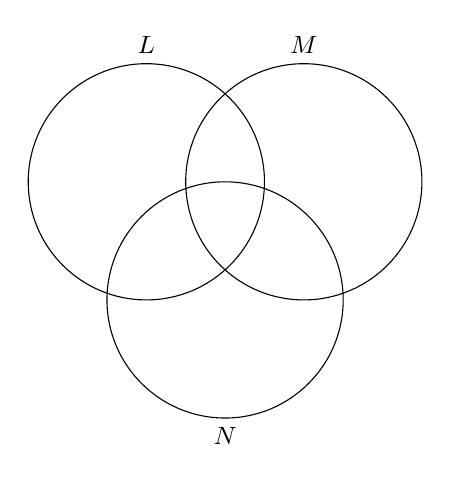
\begin{tikzpicture}[font=\small]
\draw (0,0)circle (1.5) (0,1.5) node[above] {$L$};
\draw(2,0) circle (1.5) (2,1.5) node [above]  {$M$};
\draw(1,-1.5)circle (1.5) (1,-3) node[below]{$N$};
\end{tikzpicture}

\end{center}
\end{multicols}
\end{esempio}

\begin{esempio}
\begin{multicols}{2}
 Tracciate nel riferimento cartesiano ortogonale il vettore~$\vec{v}(1;-3)$. Nella richiesta di questo quesito sembra manchi qualcosa: conosciamo
le componenti del vettore, ma dove mettiamo il primo estremo? Provate a mettere il primo estremo in ciascuno dei seguenti punti:~$A_1(-1;2)$, $A_2(1;0)$, $A_3(3;-2)$
e determinate il secondo estremo di ciascun vettore; completate indicando per ciascuno di essi il modulo e la direzione. È vero che tutti i vettori tracciati sono equipollenti?
In figura è rappresentato il vettore equipollente a quelli costruiti avente il primo estremo nell'origine del riferimento?
\begin{center}
 % (c) 2012 Dimitrios Vrettos - d.vrettos@gmail.com

\begin{tikzpicture}[x=10mm,y=10mm, font=\small]

  \begin{scope}[->]
    \draw (-1.5,0) -- (2.5,0) node [below right] () {$x$};
    \draw (0,-3.5) -- (0,1.5) node[above left] {$y$};
  \end{scope}

  \foreach \x/\xtext in {-1/-1, 1/1,2/2}{
    \node[below] at (\x,0) {$\xtext$};
    \draw (\x,1.5pt) -- (\x,-1.5pt);}
  \foreach \y/\ytext in {-3/-3,-2/-2,-1/-1, 1/1}{
    \node[left] at (0,\y) {$\ytext$};
    \draw (1.5pt,\y) -- (-1.5pt,\y);}
  \node[below left] at (0,0) {$0$};

  \begin{scope}[dotted, orange]
    \draw (-1.5,-3.5) grid (2.5,1.5);
  \end{scope}

  \begin{scope}[thick, Maroon, shorten >=1.5pt, ->]
    \draw (-0,0) -- (1,-2);
      \end{scope}
  
\begin{scope}[fill=CornflowerBlue, draw=black]
\filldraw (1,-2) circle (1.5pt) node[below right] {$B$};
\filldraw (0,0) circle (1.5pt) node[above left] {$A$};
\end{scope}

\node at (.8,-1) {$\vec{u}$};

\end{tikzpicture}
\end{center}

\end{multicols}

\osservazione
Quando si assegna un vettore (libero) mediante le sue componenti, collocheremo il primo estremo
nell'origine del riferimento cartesiano ortogonale e il secondo estremo (punta della freccia) avrà come
coordinate le componenti del vettore in questione.
\end{esempio}
\end{exrig}

\ovalbox{\risolvi \ref{ese:B.1}}

\section{Operazioni con i vettori}

\subsection{Somma di vettori}

\begin{definizione}
Nel punto~$A$ del piano sono applicati due vettori~$\vec{u}$ e~$\vec{v}$: dall'estremo~$B$ si
traccia la retta parallela ad~$AC$ e da~$C$ la parallela ad~$AB$ indicando con~$D$ il loro punto di intersezione.
Si definisce \emph{somma dei vettori}~$\vec{u}$ e~$\vec{v}$ il vettore~$\vec{w}$ individuato dalla diagonale~$AD$ del parallelogramma $ABDC$ e si scrive~$\vec{w}=\vec{u}+\vec{v}$.
\end{definizione}

\begin{figure}[h]
\centering
\input{./lbr/chapB/fig008_vet.pgf}
 \caption{Somma di due vettori.}\label{fig:F.5}
\end{figure}

Nella sua opera ``Philosophiae naturalis principia mathematica'' del~1682, Isaac Newton\footnote{matematico, fisico, filosofo, astronomo, teologo e alchimista inglese (1642 - 1727).} nel primo corollario alle leggi del moto,
scrive: <<un corpo spinto da due forze congiunte descriverà la diagonale di un parallelogramma nello stesso tempo nel quale descriverebbe separatamente i lati>>.

\vspazio\ovalbox{\risolvi \ref{ese:B.2}}

Illustriamo con un esempio che per la somma di vettori vale la proprietà associativa.

\begin{exrig}
\begin{esempio}
Dimostriamo che vale~$\vec{u}+(\vec{v}+\vec{w})=(\vec{u}+\vec{v})+\vec{w}$.

Nella figura \ref{fig:F.6} è realizzata la costruzione~$\vec{v}+\vec{w}=\vec{k}$ e~$\vec{u}+\vec{k}=\vec{j}$.
Nella figura \ref{fig:F.7} è realizzata la costruzione~$\vec{u}+\vec{v}=\vec{z}$ e~$\vec{z}+\vec{w}=\vec{j}$.
Sovrapponendo le due figure si può constatare che i due vettori~$\vec{j}$ risultanti coincidono.
\end{esempio}
\end{exrig}

\begin{figure}[t]
\begin{minipage}{.45\textwidth}
 \centering
 % (c) 2012 Dimitrios Vrettos - d.vrettos@gmail.com

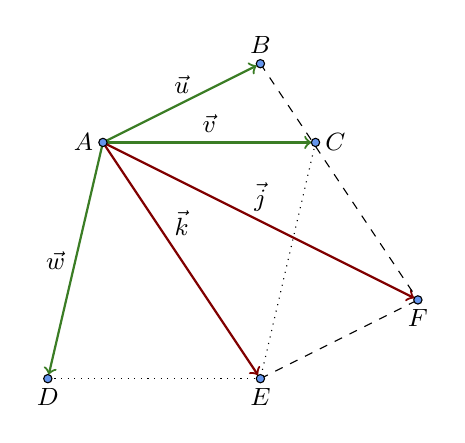
\begin{tikzpicture}[x=10mm,y=10mm, font=\small]

  \begin{scope}[thick,shorten >=1.5pt, ->]
    \begin{scope}[OliveGreen]
      \draw (0,0) -- (2,1); % vettore u
      \draw (0,0) -- (2.7,0); % vettore v
      \draw (0,0) -- (-.7,-3); % vettore w
    \end{scope}  
    
    \begin{scope}[Maroon]
      \draw (0,0) -- (4,-2); % vettore j
      \draw (0,0) -- (2,-3); % vettore k    
    \end{scope}
  \end{scope}

  \begin{scope}[dashed]
    \draw[xshift=20mm,yshift=-30mm] (0,0) -- (2,1);
    \draw[xshift=20mm,yshift=10mm] (0,0) -- (2,-3);
  \end{scope}

  \begin{scope}[dotted]
    \draw[xshift=-7mm,yshift=-30mm] (0,0) -- (2.7,0);
    \draw[xshift=27mm,yshift=0mm] (0,0) -- (-.7,-3);
  \end{scope}  

  \begin{scope}[fill=CornflowerBlue, draw=black]
    \filldraw (0,0) circle (1.5pt) node[left] {$A$};
    \filldraw (2,1) circle (1.5pt) node[above] {$B$};
    \filldraw (2,-3) circle (1.5pt) node[below] {$E$};
    \filldraw (4,-2) circle (1.5pt) node[below] {$F$};
    \filldraw (-.7,-3) circle (1.5pt) node[below] {$D$};
    \filldraw (2.7,0) circle (1.5pt) node[right] {$C$};
  \end{scope}

  \node[above] at (1,.5) {$\vec{u}$};
  \node[above] at (1.35,0) {$\vec{v}$};
  \node[above] at (2,-1) {$\vec{j}$};
  \node[above] at (1,-1.3) {$\vec{k}$};
  \node at (-.6,-1.5) {$\vec{w}$};

\end{tikzpicture}
 \caption{$\vec{v}+\vec{w}=\vec{k}$ e~$\vec{u}+\vec{k}=\vec{j}$.}
 \label{fig:F.6}
\end{minipage}\hfil
\begin{minipage}{.45\textwidth}
 \centering
 % (c) 2012 Dimitrios Vrettos - d.vrettos@gmail.com

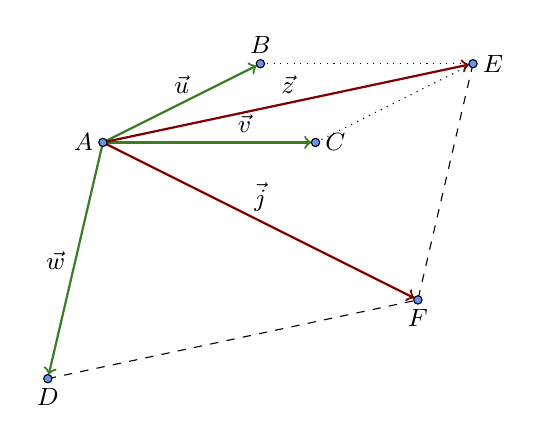
\begin{tikzpicture}[x=10mm,y=10mm, font=\small]

  \begin{scope}[thick,shorten >=1.5pt, ->]
    \begin{scope}[OliveGreen]
      \draw (0,0) -- (2,1); % vettore u
      \draw (0,0) -- (2.7,0); % vettore v
      \draw (0,0) -- (-.7,-3); % vettore w
    \end{scope}
    
    \begin{scope}[Maroon]
      \draw (0,0) -- (4,-2); % vettore j
      \draw (0,0) -- (4.7,1); % vettore z    
    \end{scope}
  \end{scope}

  \begin{scope}[dashed]
    \draw[xshift=47mm,yshift=10mm] (0,0) -- (-.7,-3);
    \draw[xshift=-7mm,yshift=-30mm] (0,0) -- (4.7,1);
  \end{scope}

  \begin{scope}[dotted]
    \draw[xshift=20mm,yshift=10mm] (0,0) -- (2.7,0);
    \draw[xshift=27mm,yshift=0mm] (0,0) -- (2,1);
  \end{scope}  

  \begin{scope}[fill=CornflowerBlue, draw=black]
    \filldraw (0,0) circle (1.5pt) node[left] {$A$};
    \filldraw (2,1) circle (1.5pt) node[above] {$B$};
    \filldraw (4.7,1) circle (1.5pt) node[right] {$E$};
    \filldraw (4,-2) circle (1.5pt) node[below] {$F$};
    \filldraw (-.7,-3) circle (1.5pt) node[below] {$D$};
    \filldraw (2.7,0) circle (1.5pt) node[right] {$C$};
  \end{scope}

  \node[above] at (1,.5) {$\vec{u}$};
  \node[above] at (1.8,0) {$\vec{v}$};
  \node[above] at (2,-1) {$\vec{j}$};
  \node[above] at (2.35,.5) {$\vec{z}$};
  \node at (-.6,-1.5) {$\vec{w}$};

\end{tikzpicture}
 \caption{$\vec{u}+\vec{v}=\vec{z}$ e~$\vec{z}+\vec{w}=\vec{j}$.}
 \label{fig:F.7}
\end{minipage}
\end{figure}

Osserviamo che la validità della proprietà associativa ci permette di costruire la somma di più vettori. Per come è definita l'operazione di somma, pensando al
vettore come rappresentante di uno spostamento dal primo estremo al secondo, possiamo interpretare la figura \ref{fig:F.5} come lo spostamento di un punto prima
da~$A$ fino a~$B$ e poi da questo fino a~$D$, essendo~$\overrightarrow{BD}$ un vettore equipollente ad~$\overrightarrow{AC}$ (cambia soltanto il punto di applicazione). Quindi possiamo affermare che il vettore somma
di due vettori~$\vec{u}$ e~$\vec{v}$ si può determinare prendendo due vettori~$\overrightarrow{AB}$ e~$\overrightarrow{BC}$ rispettivamente equipollenti
ai dati; se~$\overrightarrow{AB} \equiv \vec{u}$ e~$\overrightarrow{BC} \equiv \vec{v}$ allora la somma è il vettore~$\overrightarrow{AC}$ avente~$A$
come primo estremo e~$C$
come secondo estremo (figura \ref{fig:F.8}).

Pertanto la somma di più vettori si può semplicemente determinare scegliendo per ogni addendo il vettore equipollente avente il primo estremo nell'estremo finale
dell'addendo precedente: la somma è il vettore avente il primo estremo nel punto iniziale del primo addendo e l'estremo finale nel secondo estremo dell'ultimo addendo.
\begin{exrig}
\begin{esempio}
Somma di più vettori:~$\vec{z}+\vec{a}+\vec{b}+\vec{c}=\vec{s}$~~(figura \ref{fig:F.9}).
\end{esempio}
\end{exrig}

\begin{figure}[hb]
\begin{minipage}[t]{.45\textwidth}
 \centering
 % (c) 2012 Dimitrios Vrettos - d.vrettos@gmail.com

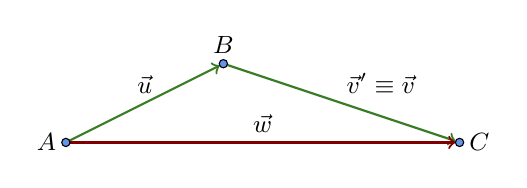
\begin{tikzpicture}[x=10mm,y=10mm, font=\small]

  \begin{scope}[thick,shorten >=1.5pt, ->]
    \begin{scope}[OliveGreen]
      \draw (0,0) -- (2,1);
      \draw (2,1) -- (5,0);
    \end{scope}  
    
    \begin{scope}[Maroon]
      \draw (0,0) -- (5,0);
    \end{scope}
  \end{scope}


  \begin{scope}[fill=CornflowerBlue, draw=black]
    \filldraw (5,0) circle (1.5pt) node[right] {$C$};
    \filldraw (0,0) circle (1.5pt) node[left] {$A$};
    \filldraw (2,1) circle (1.5pt) node[above] {$B$};
  \end{scope}

  \node[above] at (1,0.5) {$\vec{u}$};
  \node[above] at (4,0.5) {$\vec{v}' \equiv \vec{v}$};
  \node[above] at (2.5,0) {$\vec{w}$};

\end{tikzpicture}
 \caption{Somma di due vettori.}
 \label{fig:F.8}
\end{minipage}\hfil
\begin{minipage}[t]{.45\textwidth}
 \centering
 % (c) 2012 Dimitrios Vrettos - d.vrettos@gmail.com

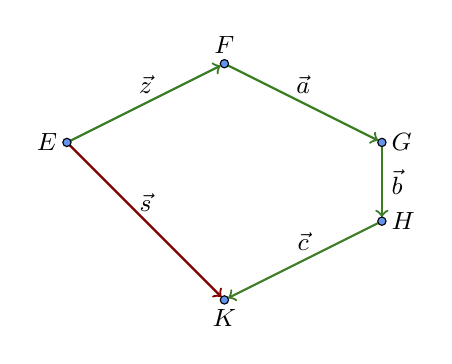
\begin{tikzpicture}[x=10mm,y=10mm, font=\small]

  \begin{scope}[thick,shorten >=1.5pt, ->]
    \begin{scope}[OliveGreen]
\draw (-2,2) -- (0,3);
\draw (0,3) -- (2,2);
\draw (2,2) -- (2,1);
\draw (2,1) -- (0,0);
    \end{scope}  
    
    \begin{scope}[Maroon]
      \draw (-2,2) -- (0,0);
    \end{scope}
  \end{scope}


  \begin{scope}[fill=CornflowerBlue, draw=black]
    \filldraw (-2,2) circle (1.5pt) node[left] {$E$};
    \filldraw (0,3) circle (1.5pt) node[above] {$F$};
    \filldraw (2,2) circle (1.5pt) node[right] {$G$};
    \filldraw (2,1) circle (1.5pt) node[right] {$H$};
    \filldraw (0,0) circle (1.5pt) node[below] {$K$};
  \end{scope}

  \node[above] at (-1,2.5) {$\vec{z}$};
  \node[above] at (1,2.5) {$\vec{a}$};
  \node[right] at (2,1.5) {$\vec{b}$};
  \node[above] at (1,.5) {$\vec{c}$};
  \node[above] at (-1,1) {$\vec{s}$};

\end{tikzpicture}
 \caption{Somma di più vettori.}
 \label{fig:F.9}
\end{minipage}
\end{figure}

Abbiamo visto come si costruisce geometricamente il vettore somma di vettori; vediamo come si determinano le componenti del vettore somma se la questione
è posta nel riferimento cartesiano ortogonale.

\begin{exrig}
\begin{esempio}
Nel piano dotato di riferimento cartesiano ortogonale costruiamo il vettore somma dei vettori~$\vec{u}(1;2)$ e~$\vec{v}(3;-1)$ e determiniamone
le componenti (figura~\ref{fig:F.10}).

Strategia risolutiva:
\begin{enumeratea}
\item posizioniamo i vettori~$\vec{u}$ e~$\vec{v}$ con il punto di applicazione nell'origine del sistema cartesiano;
\item costruiamo il vettore~$\vec{w}$ equipollente al vettore~$\vec{v}$ applicato al punto~$A$;
\item determiniamo il punto	$D(4;1)$;
\item costruiamo il vettore~$\vec{z}=\vec{u}+\vec{v}$ di coordinate~$\vec{z}(4;1)$.
\end{enumeratea}
Osserviamo che il primo passo realizzato ci permette di affermare~$x_z=x_u+x_v$ e~$y_z=y_u+y_v$.
\end{esempio}
\end{exrig}
%\newpage
\begin{figure}[t]
\centering
% (c) 2012 Dimitrios Vrettos - d.vrettos@gmail.com

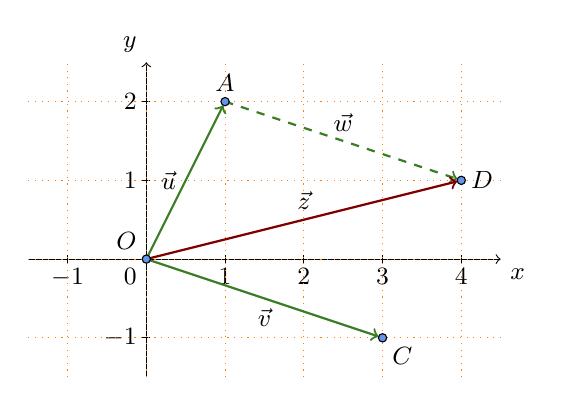
\begin{tikzpicture}[x=10mm,y=10mm, font=\small]

  \begin{scope}[->]
    \draw (-1.5,0) -- (4.5,0) node [below right] () {$x$};
    \draw (0,-1.5) -- (0,2.5) node[above left] {$y$};
  \end{scope}

  \foreach \x/\xtext in {-1/-1, 1/1,2/2,3/3,4/4}{
    \node[below] at (\x,0) {$\xtext$};
    \draw (\x,1.5pt) -- (\x,-1.5pt);}
  \foreach \y/\ytext in {-1/-1, 1/1,2/2}{
    \node[left] at (0,\y) {$\ytext$};
    \draw (1.5pt,\y) -- (-1.5pt,\y);}
  \node[below left] at (0,0) {$0$};

  \begin{scope}[dotted, orange]
    \draw (-1.5,-1.5) grid (4.5,2.5);
  \end{scope}

  \begin{scope}[thick, shorten >=1.5pt, ->]
  
	\draw[OliveGreen] (0,0) -- (1,2);
	\draw[OliveGreen] (0,0) -- (3,-1);
	\draw[OliveGreen, dashed] (1,2) -- (4,1);  
	\draw[Maroon] (-0,0) -- (4,1);
      \end{scope}
  
\begin{scope}[fill=CornflowerBlue, draw=black]
\filldraw (1,2) circle (1.5pt) node[above] {$A$};
\filldraw (0,0) circle (1.5pt) node[above left] {$O$};
\filldraw (4,1) circle (1.5pt) node[right] {$D$};
\filldraw (3,-1) circle (1.5pt) node[below right] {$C$};
\end{scope}

\node[left] at (.5,1) {$\vec{u}$};
\node[above] at (2.5,1.5) {$\vec{w}$};
\node[above] at (2,.5) {$\vec{z}$};
\node[below] at (1.5,-.5) {$\vec{v}$};
\end{tikzpicture}
\caption{Determinazione delle componenti di un vettore.}\label{fig:F.10}
\end{figure}

\begin{procedura} Note le componenti cartesiane dei vettori addendi~$\vec{u}=(x_u;y_u)$ e~$\vec{v}=(x_v;y_v)$ le
 componenti cartesiane del vettore somma~$\vec{z}=(x_z;y_z)$ si ottengono con la regola del parallelogramma:

Il primo passo realizzato nella costruzione precedente ci permette di affermare che le componenti del vettore somma $\vec{z}$ sono la somma
delle componenti dei vettori addendi:\[x_z=x_u+x_v\quad\text{e}\quad y_z=y_u+y_v.\]
\end{procedura}

\ovalbox{\risolvi \ref{ese:B.3}}

\paragraph{Applicazioni dei vettori}
I vettori sono degli enti geometrici che vengono spesso utilizzati in fisica per rappresentare tutte le grandezze che sono definite conoscendo modulo, direzione,
verso e punto di applicazione. Esempi di grandezze vettoriali sono: la velocità, l'accelerazione, la forza, il campo elettrico.

\begin{exrig}
\begin{esempio}
Nella figura seguente sono rappresentate tre scatole viste dall'alto e su ognuna di esse agiscono due forze, come rappresentato in figura. Calcola la forza risultante $\vec{r}$ in ognuno dei casi,
sapendo che una forza ha modulo~$4 \unit{N}$ e l'altra~$9 \unit{N}$.
\begin{center}
 % (c) 2012 Dimitrios Vrettos - d.vrettos@gmail.com

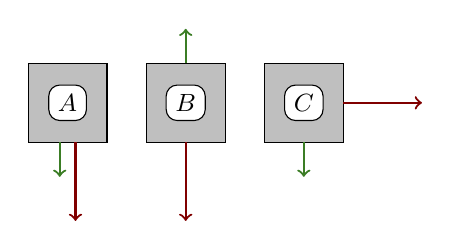
\begin{tikzpicture}[x=10mm,y=10mm, font=\small]

  \begin{scope}[fill=lightgray, draw=black]
    \foreach \x in {0, 1.5, 3}
      \filldraw (\x,0) rectangle  (\x+1,1);
  \end{scope}

  \begin{scope}[every node/.style={fill=white,rectangle, rounded corners, draw=black}]
    \foreach \x/\xtext in {.5/A,2/B,3.5/C}
      \node at (\x,.5) {$\xtext$};
  \end{scope}

  \begin{scope}[thick, ->]
    \begin{scope}[Maroon]
      \draw (.6,0) -- (.6,-1);
      \draw (2,0) -- (2,-1);
      \draw (4,.5) -- (5,.5);
    \end{scope}

    \begin{scope}[OliveGreen]
      \draw (.4,0) -- (.4,-.44);
      \draw (2,1) -- (2,1.44);
      \draw (3.5,0) -- (3.5,-.44);
    \end{scope}
  \end{scope}
\end{tikzpicture}
\end{center}
\newpage
\emph{Svolgimento:}
\begin{enumeratea}
\item Nel primo caso ($A$) i due vettori hanno la stessa direzione e lo stesso verso, quindi la risultante si ottiene addizionando semplicemente i due moduli:~$|\vec{r}|=4 +9 =13 \unit{N}$;
\item Nel secondo caso ($B$) poiché i vettori sono opposti come verso, si procede sottraendo al vettore maggiore il vettore minore e la forza risultante ha la direzione ed il verso
del vettore di modulo maggiore:~$|\vec{r}|=9 - 5 =4 \unit{N}$.
\item Nel terzo caso ($C$) i due vettori hanno direzioni perpendicolari, quindi il vettore somma si ottiene con il metodo del parallelogramma. Il suo modulo si ottiene applicando il teorema di Pitagora:
\[|\vec{r}|=\sqrt{4^2+9^2}=\sqrt{97}\simeq \np[N]{9,85}.\]
\end{enumeratea}
\end{esempio}
\end{exrig}

\subsection{Differenza tra vettori}

\begin{procedura} Per determinare la \emph{differenza tra due vettori} (figura~\ref{fig:F.11}) $\vec{u}$ e~$\vec{v}$
si procede nel seguente modo:
\begin{enumeratea}
\item costruiamo il vettore~$\vec{z}=-\vec{v}$ che ha stessa direzione, stesso modulo, ma verso opposto;
\item determiniamo con la regola del parallelogramma~$\vec{w}=\vec{u}+\vec{z}$.
\end{enumeratea}
Il vettore ottenuto è la differenza tra i vettori assegnati:~$\vec{w}=\vec{u}-\vec{v}$.
\end{procedura}

\begin{figure}[htb]
 \centering
 % (c) 2012 Dimitrios Vrettos - d.vrettos@gmail.com

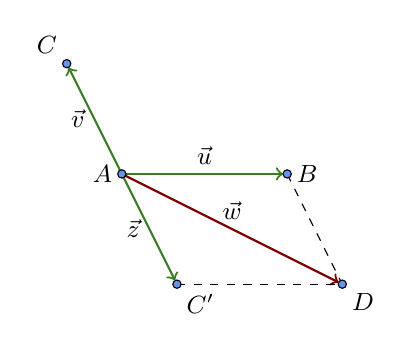
\begin{tikzpicture}[x=7mm,y=7mm, font=\small]

 \begin{scope}[thick, shorten >=1.5pt, ->]
  
	\draw[OliveGreen] (0,0) -- (-1,2);
	\draw[OliveGreen] (0,0) -- (1,-2);
	\draw[OliveGreen] (0,0) -- (3,0);  
	\draw[Maroon] (0,0) -- (4,-2);
      \end{scope}
  
\begin{scope}[dashed]
\draw (3,0) -- (4,-2);
\draw (1,-2) -- (4,-2);
\end{scope}
\begin{scope}[fill=CornflowerBlue, draw=black]
\filldraw (0,0) circle (1.5pt) node[left] {$A$};
\filldraw (3,0) circle (1.5pt) node[right] {$B$};
\filldraw (4,-2) circle (1.5pt) node[below right] {$D$};
\filldraw (1,-2) circle (1.5pt) node[below right] {$C'$};
\filldraw (-1,2) circle (1.5pt) node[above left] {$C$};
\end{scope}

\node[above] at (1.5,0) {$\vec{u}$};
\node[above] at (2,-1) {$\vec{w}$};
\node[left] at (.5,-1) {$\vec{z}$};
\node[left] at (-.5,1) {$\vec{v}$};
\end{tikzpicture}
 \caption{Differenza di due vettori.}
 \label{fig:F.11}
\end{figure}

\begin{exrig}
\begin{esempio}

Sono assegnati i vettori~$\vec{u}(4;0)$ e~$\vec{v}(-2;-1)$. Determinare~$\vec{d_1}=\vec{u}-\vec{v}$ e~$\vec{d_2}=\vec{v}-\vec{u}$. Cosa osservate?
\begin{center}
 % (c) 2012 Dimitrios Vrettos - d.vrettos@gmail.com

\begin{tikzpicture}[x=10mm,y=10mm, font=\small, every state/.style={draw=CornflowerBlue, minimum size=0pt}]

\node[state] (X) at (-1,0) {$X$};
\node[state] (H) at (.5,.5) {$H$};
\node[state] (K) at (1,-1) {$K$};
\node[state] (Z) at (-.5,-1) {$Z$};

\begin{scope}[->, Maroon]
\draw (X)--(H);
\draw (X)--(Z);
\draw (H)--(K);
\end{scope}

\end{tikzpicture}

\end{center}
\end{esempio}
\end{exrig}

\subsection{Moltiplicazione di un numero reale per un vettore}

\begin{definizione}
Assegnato un numero reale~$r$ ed un vettore~$\vec{v}$, il \emph{prodotto}
\[\vec{p} = r \cdot \vec{v}\]
è un vettore avente:
\begin{enumeratea}
\item la stessa direzione del vettore~$\vec{v}$;
\item intensità o modulo uguale al prodotto del modulo di~$\vec{v}$ per il valore assoluto di~$r$:
 \subitem $|\vec{p}|=|r| \cdot|\vec{v}|$;
\item verso uguale al verso di~$\vec{v}$ se~$r$ è positivo, verso opposto a quello di~$\vec{v}$ se~$r$ è negativo.
\end{enumeratea}
\end{definizione}

\begin{exrig}
\begin{esempio}
Nella figura sono rappresentati il vettore~$\vec{v}$ e altri vettori ottenuti moltiplicandolo per un numero reale:
$\vec{a}=2 \cdot \vec{v}$,~~$\vec{b}=-\dfrac{3}{2} \cdot \vec{v}$,~~$\vec{c}=\dfrac{1}{3} \cdot \vec{v}$.
\begin{center}
 % (c) 2012 Dimitrios Vrettos - d.vrettos@gmail.com

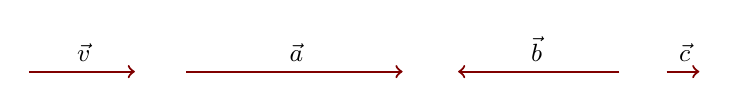
\begin{tikzpicture}[x=7mm,y=7mm, font=\small]

 \begin{scope}[thick, shorten >=1.5pt, ->, Maroon]
	\draw (0,0) -- (2,0); %vettore v
\node[above, black] at (1,0) {$\vec{v}$};
	\begin{scope}[xshift=20mm]
	\draw (0,0) -- (4,0); %vettore a
\node[above, black] at (2,0) {$\vec{a}$};
	\end{scope}
	\begin{scope}[xshift=54mm]
	\draw (3,0) -- (0,0); %vettore b
\node[above, black] at (1.5,0) {$\vec{b}$};
	\end{scope}
	\begin{scope}[xshift=81mm]
	\draw (0,0) -- (.67,0); %vettore c
\node[above, black] at (.33,0) {$\vec{c}$};
	\end{scope}
\end{scope}

\end{tikzpicture}
\end{center}

\end{esempio}
\begin{esempio}
Nel piano dotato di riferimento cartesiano ortogonale rappresentiamo il vettore~$\vec{u}(4;1)$; le componenti
del vettore~$\vec{p}=-2\cdot \vec{u}$ si ottengono moltiplicando per~$-2$ le componenti del vettore dato:~$\vec{p}(-8;-2)$. $\vec{p}$ e~$\vec{u}$
hanno la stessa direzione essendo~$m_{\vec{u}}=\frac{1}{4}=m_{\vec{p}}$ e anzi appartengono alla stessa retta avendo in comune il punto di applicazione $O(0;0)$.
\begin{center}
 % (c) 2012 Dimitrios Vrettos - d.vrettos@gmail.com

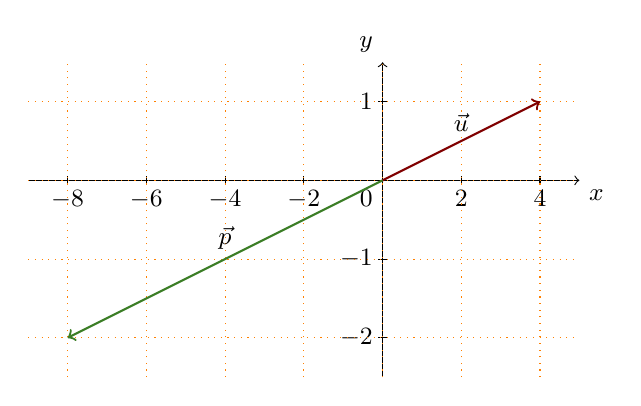
\begin{tikzpicture}[x=10mm,y=10mm, font=\small]

  \begin{scope}[->]
    \draw (-4.5,0) -- (2.5,0) node [below right] () {$x$};
    \draw (0,-2.5) -- (0,1.5) node[above left] {$y$};
  \end{scope}

  \foreach \x/\xtext in {-4/-8, -3/-6,-2/-4,-1/-2,1/2,2/4}{
    \node[below] at (\x,0) {$\xtext$};
    \draw (\x,1.5pt) -- (\x,-1.5pt);}
  \foreach \y/\ytext in {-2/-2,-1/-1, 1/1}{
    \node[left] at (0,\y) {$\ytext$};
    \draw (1.5pt,\y) -- (-1.5pt,\y);}
  \node[below left] at (0,0) {$0$};

  \begin{scope}[dotted, orange]
    \draw (-4.5,-2.5) grid (2.5,1.5);
  \end{scope}

  \begin{scope}[thick, ->]
	\draw[Maroon] (0,0) -- (2,1);  
	\draw[OliveGreen](0,0) -- (-4,-2);
      \end{scope}
 
\node[above] at (1,.5) {$\vec{u}$};
\node[above] at (-2,-1) {$\vec{p}$};
\end{tikzpicture}
\end{center}
\end{esempio}
\end{exrig}

In generale, dato un vettore~$\vec{u}(x_u;y_u)$ si ha che~$r \cdot \vec{u} = \vec{p}(r \cdot x_u; r \cdot y_u)$, quindi la sua direzione è $m_{\vec{p}}=\frac{r \cdot y_u}{r \cdot x_u}=\frac{y_u}{x_u}= m_{\vec{u}}$, cioè la stessa di $\vec{u}$.

\begin{osservazione}
Se due vettori hanno la stessa direzione, cioè appartengono a rette parallele, si può sempre trovare un numero reale~$r$
tale che uno sia~$r$ volte l'altro. La figura seguente può suggerirvi come giustificare l'osservazione precedente.
\begin{center}
 % (c) 2012 Dimitrios Vrettos - d.vrettos@gmail.com

\begin{tikzpicture}[x=10mm,y=10mm, font=\small]

  \begin{scope}[->, thick]
\draw[OliveGreen] (0,0) -- (4,0);
\draw[Maroon] (1,1) -- (3,1);
\end{scope}
\node[above] at (2,1) {$\vec{u}$};
\node[above] at (2,0) {$\vec{v}$};
\begin{scope}[dotted]
\draw (0,0) -- (2,2)--(4,0);
\end{scope}
\end{tikzpicture}
\end{center}
\end{osservazione}

\begin{exrig}
\begin{esempio}

Sono assegnati i vettori~$\vec{x}(\frac {1}{2};1)$, $\vec{y}(-3;-1)$ e $\vec{z}(0;3)$.
Costruite i vettori~$\vec{p_1}=2 \cdot \vec{x}-\vec{y}$,~~$\vec{p_2}=2 \cdot (\vec{z}+\vec{y})$,~~$\vec{p_3}=-\frac {3}{2} \cdot \vec{z} +2 \cdot \vec{y}+3 \cdot \vec{x}$
e determinatene le componenti.
\end{esempio}
\end{exrig}


\ovalbox{\risolvii \ref{ese:B.4}, \ref{ese:B.5}, \ref{ese:B.6}}

\section{Dipendenza e indipendenza lineare}

\begin{definizione}
Diciamo che un vettore~$\vec{v}$ è \emph{combinazione lineare} di altri vettori~$\vec{x}$, $\vec{y}$, $\vec{z}$ se esistono
i numeri reali~$r_1$, $r_2$, $r_3$, detti \emph{coefficienti della combinazione lineare}, per i quali risulta verificata
l'uguaglianza~$\vec{v}=r_1 \cdot \vec{x} + r_2 \cdot \vec{y} + r_3 \cdot \vec{z}$.
\end{definizione}
%\newpage
\begin{exrig}
\begin{esempio}
Nell'esempio precedente hai costruito i vettori~$\vec{p_1}$, $\vec{p_2}$, $\vec{p_3}$ eseguendo la somma algebrica di vettori costruiti moltiplicando
per numeri reali i vettori assegnati~$\vec{x}$, $\vec{y}$, $\vec{z}$. Possiamo dire che:
\begin{itemize*}
\item $\vec{p_1}$ è combinazione lineare dei vettori~$\vec{x}$ e~$\vec{y}$ i cui coefficienti sono~$r_1=2$, $r_2=-1$.
\item $\vec{p_2}$ è combinazione lineare dei vettori~$\vec{z}$ e~$\vec{y}$ i cui coefficienti sono~$r_1=2$, $r_2=2$.
\item $\vec{p_3}$ è combinazione lineare dei vettori~$\vec{x}$, $\vec{y}$ e~$\vec{z}$ i cui coefficienti sono~$r_1=-\frac{3}{2}$, $r_2=2$ e $r_3=3$.
\end{itemize*}
\end{esempio}
\end{exrig}

Nell'insieme~$\spV$ di tutti i vettori del piano cartesiano, consideriamo i vettori~$\vec{i}(1;0)$ e~$\vec{j}(0;1)$ appartenenti
rispettivamente all'asse delle ascisse e a quello delle ordinate; possiamo notare che $\vec{i}$ e $\vec{j}$ formano tra loro un angolo di $90\grado$ e che $|\vec{i}|=|\vec{j}|=1$. Tali vettori sono chiamati \emph{versori} associati rispettivamente dell'asse $x$ e all'asse $y$.

Ogni vettore~$\vec{v}$ del piano può essere scritto come combinazione lineare di~$\vec{i}$ e~$\vec{j}$ e le sue componenti sono i coefficienti
della combinazione lineare di $\vec{i}$ e $\vec{j}$ con i quali si determina~$\vec{v}$.
\[\vec{v}(x_v;y_v)=x_v \cdot \vec{i}+y_v \cdot \vec{j}\]

\ovalbox{\risolvi \ref{ese:B.7}}

\begin{exrig}
\begin{esempio}
Disegniamo nel riferimento cartesiano ortogonale i vettori~$\vec{u}(1;1)$, $\vec{v}(4;-2)$, $\vec{w}(3;1)$; ci chiediamo se è possibile scrivere~$\vec{w}$
come combinazione lineare degli altri due.
\begin{center}
 % (c) 2012 Dimitrios Vrettos - d.vrettos@gmail.com

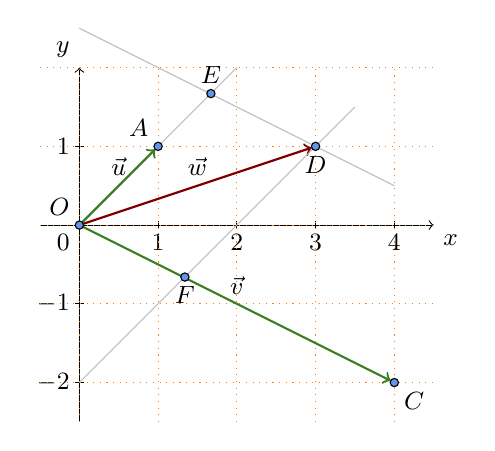
\begin{tikzpicture}[x=10mm,y=10mm, font=\small]

  \begin{scope}[->]
    \draw (-.5,0) -- (4.5,0) node [below right] {$x$};
    \draw (0,-2.5) -- (0,2) node[above left] {$y$};
  \end{scope}

  \foreach \x/\xtext in {1/1,2/2,3/3,4/4}{
    \node[below] at (\x,0) {$\xtext$};
    \draw (\x,1.5pt) -- (\x,-1.5pt);}
  \foreach \y/\ytext in {-2/-2,-1/-1, 1/1}{
    \node[left] at (0,\y) {$\ytext$};
    \draw (1.5pt,\y) -- (-1.5pt,\y);}
  \node[below left] at (0,0) {$0$};

  \begin{scope}[dotted, orange]
    \draw (-.5,-2.5) grid (4.5,2);
  \end{scope}

  \begin{scope}[thick, ->,shorten >=1.5pt]
	\draw[Maroon] (0,0) -- (3,1);     % OD
	\draw[OliveGreen](0,0) -- (1,1);  % OA
	\draw[OliveGreen](0,0) -- (4,-2); % OC
      \end{scope}
 
\begin{scope}[lightgray]
\draw (1,1) -- (2,2);
\draw[xshift=20mm] (-2,-2) -- (1.5,1.5);
\draw[yshift=25mm](0,0)--(4,-2);
\end{scope}

\begin{scope}[fill=CornflowerBlue, draw=black]
\filldraw (0,0) circle (1.5pt)node [above left]{$O$};
\filldraw (3,1) circle (1.5pt)node [below]{$D$};
\filldraw (1,1) circle (1.5pt)node [above left]{$A$};
\filldraw (1.34,-.66) circle (1.5pt)node [below]{$F$};
\filldraw (1.67,1.67) circle (1.5pt) node [above]{$E$};
\filldraw (4,-2) circle (1.5pt) node [below right]{$C$};
\end{scope}

\node[above] at (0.5,0.5) {$\vec{u}$};
\node[above] at (2,-1) {$\vec{v}$};
\node[above] at (1.5,0.5) {$\vec{w}$};

\end{tikzpicture}
\end{center}


\paragraph{Il metodo geometrico} Dobbiamo costruire due vettori~$\vec{u}'=r_1 \cdot \vec{u}$ e~$\vec{v}'=r_2 \cdot \vec{v}$ tali che sommati diano
il vettore~$\vec{w}$. Dal punto~$D$ tracciamo la parallela alla retta~$OC$, che interseca la retta~$AO$ nel punto~$E$; dallo stesso punto~$D$
tracciamo la parallela alla retta~$AO$ che interseca in~$F$ la retta~$OC$. I punti~$E$ ed~$F$ sono gli
estremi dei due vettori~$\vec{u}'$ e $\vec{v}'$ cercati: $\vec{u}'=\overrightarrow{OE}=r_1 \cdot \vec{u}$ e~$\vec{v}'=\overrightarrow{OF}=r_2 \cdot \vec{v}$ con~$r_1>1$ e~$r_2<1$ rispettivamente ottenuti
allungando e accorciando~$\vec{u}$ e~$\vec{v}$. Si ha quindi~$\vec{w}=r_1 \cdot \vec{u} + r_2 \cdot \vec{v}$.

\paragraph{Il metodo algebrico} Dobbiamo trovare due numeri~$r_1$ e~$r_2$ tali che
\[ \vec{w}=r_1 \cdot \vec{u}+r_2 \cdot \vec{v} \quad\Rightarrow\quad
\left\{\begin{array}{l}
3=1 \cdot r_1+1 \cdot r_2 \quad\text{(componenti }x\text{)} \\
1=1 \cdot r_1-2 \cdot r_2 \quad\text{(componenti }y\text{)}
\end{array}\right. \]
%\newpage
e risolvendo il sistema lineare di due equazioni in due incognite si ottiene~$r_1=\frac{5}{3}$ e~$r_2=\frac{1}{3}$, coerentemente ai risultati della costruzione geometrica effettuata.
\end{esempio}
\end{exrig}

\ovalbox{\risolvi \ref{ese:B.8}}

\begin{definizione}
Dati $n$ vettori $\vec{v}_1$, $\vec{v}_2$, \ldots, $\vec{v}_n$, questi si dicono \emph{linearmente indipendenti} se almeno uno di essi si può scrivere come combinazione lineare degli altri. Se nessuno degli $n$ vettori $\vec{v}_1$, $\vec{v}_2$, \ldots, $\vec{v}_n$ può essere scritto come combinazione lineare degli altri, i vettori si dicono \emph{linearmente indipendenti}.
\end{definizione}

\vspazio\ovalbox{\risolvii \ref{ese:B.9}, \ref{ese:B.10}}

\newpage
% (c) 2012 Tiziana Manca - tmanca@libero.it
% (c) 2012-2014 Dimitrios Vrettos - d.vrettos@gmail.com
%===================================
\section{Esercizi}
%===================================
\subsection{Esercizi dei singoli paragrafi}
%===================================
\subsubsection*{\thechapter.1 - Proposizioni e predicati}

\begin{esercizio}
\label{ese:B.1}
Completa la tabella come suggerito nella prima riga, individuando, per ciascuna proposizione, il predicato e gli argomenti a cui esso si riferisce:
\begin{center}
\begin{tabular}{llc}
\toprule
Proposizioni & Predicato & Argomenti\\
\midrule
7 è divisore di~14 & essere divisore di & 7, 14 \\
11 è maggiore di~10 & essere maggiore di & \\
5 è numero primo & & \\
Andrea frequenta la stessa palestra di Marco & & \\
Marta è moglie di Piero & & \\
Paolo è padre di Marco & & \\
\bottomrule
\end{tabular}
\end{center}
\end{esercizio}


\begin{multicols}{2}
%===================================
\subsubsection*{\thechapter.2 - Relazioni in un insieme}
\begin{esercizio}
\label{ese:B.2}
Nell'insieme~$A = \{$3, 5, 6, 9, 30$\}$ considera il predicato ``essere minore di''; con esso forma proposizioni vere aventi come soggetto e come complemento due elementi di~$A$.
\begin{enumeratea}
\item $p_1$: 9\text{ è minore di }30;
\item $p_2$: \dotfill;
\item $p_3$: \dotfill
\end{enumeratea}
\end{esercizio}

\begin{esercizio}
\label{ese:B.3}
Nell'insieme~$A$ rappresentato con il diagramma di Eulero-Venn di figura~\ref{fig:B.11} a pagina~\pageref{fig:B.11} introduciamo il predicato~$\Rel$: ``avere
una sola lettera diversa''. Costruisci l'insieme~$G_\Rel$.

\emph{Traccia di soluzione}:
Per costruire l'insieme~$G_\Rel$ devo formare le coppie ordinate ricordando che per qualunque~$a$ e~$b$ appartenenti ad~$A$, $a \,\Rel\, b$
se e solo se ``$a$ ha una sola lettera diversa da~$b$'', ad esempio prete$\,\Rel\,$prese.
\end{esercizio}

\begin{esercizio}
\label{ese:B.4}
Nell'insieme~$C = \{$Como, Milano, Venezia, Parma, Brescia, Aosta, Torino, Genova, Imperia, Arezzo,
Firenze, Grosseto, Napoli, Campobasso, Catanzaro, Bologna, Vercelli, Salerno$\}$ è definita la
relazione~$\Rel$: ``essere nella stessa regione''. Costruisci l'insieme~$G_\Rel$.
\end{esercizio}

\begin{esercizio}
\label{ese:B.5}
Nell'insieme~$S = \{ x \mid  x$ è il nome di un giorno della settimana$\}$ è definita la
relazione~$\Rel$:~$x \in S$, $y \in S$, $x \,\Rel\, y$ se e solo se ``$x$ ha
lo stesso numero di sillabe di~$y$''. Costruisci l'insieme~$G_\Rel$.
\end{esercizio}

\begin{esercizio}
\label{ese:B.6}
Nell'insieme~$F = \{$1, 3, 4, 6, 5, 9, 0, 2$\}$ è definita la relazione~$\Rel$: ``essere consecutivi''. Costruisci l'insieme~$G_\Rel$.
\end{esercizio}
\end{multicols}

\begin{figure}[t]
\begin{minipage}[b]{.45\textwidth}
 \centering
 % (c) 2012 Dimitrios Vrettos - d.vrettos@gmail.com

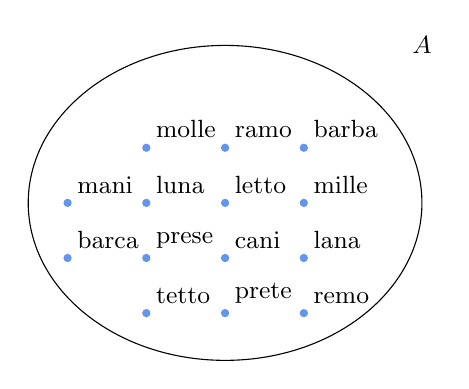
\begin{tikzpicture}[x=10mm,y=10mm, font=\small]
\draw (0,0) circle [x radius=2.5, y radius=2];

\node  at (2.5,2) {$A$};
 \begin{scope}[fill=CornflowerBlue]
\fill (0,0) circle (1.5pt) node[above right] {letto};
\fill (-1,0) circle (1.5pt) node[above right] {luna};
\fill (-2,0) circle (1.5pt) node[above right] {mani};
\fill (-2,-.7) circle (1.5pt) node[above right] {barca};
\fill (1,0) circle (1.5pt) node[above right] {mille};
\fill (0,.7) circle (1.5pt) node[above right] {ramo};
\fill (1,.7) circle (1.5pt) node[above right] {barba};
\fill (-1,.7) circle (1.5pt) node[above right] {molle};
\fill (0,-.7) circle (1.5pt) node[above right] {cani};
\fill (1,-.7) circle (1.5pt) node[above right] {lana};
\fill (-1,-.7) circle (1.5pt) node[above right] {prese}; 
\fill (0,-1.4) circle (1.5pt) node[above right] {prete};
\fill (1,-1.4) circle (1.5pt) node[above right] {remo};
\fill (-1,-1.4) circle (1.5pt) node[above right] {tetto}; 
 \end{scope}
\end{tikzpicture}
 \caption{Esercizio \ref{ese:B.3}.}\label{fig:B.11}
\end{minipage}\hfil
\begin{minipage}[b]{.45\textwidth}
 \centering
 % (c) 2012 Dimitrios Vrettos - d.vrettos@gmail.com
\begin{tikzpicture}[scale=.5, x=7.5mm, y=7.5mm, font=\scriptsize]
\begin{scope}[->]
\draw (0,0) -- (0,7.5);
\draw (0,0) -- (7.5,0);
\end{scope}

\begin{scope}[Maroon, dotted, step=7.5mm]
\draw (0,0) grid (7.5,7.5);
\end{scope}

\foreach \x/\xtext in {1/lunedì,2/martedì}{
\node[below left=.2, rotate=30] at (\x,0) {\xtext};
\node[left=.15] at (0,\x) {\xtext};
}
\begin{scope}[very thick, draw=CornflowerBlue, decoration={crosses, shape size=1.5mm}]
\draw decorate {(1,1) -- (1,1.1)};
\draw decorate {(2,2) -- (2,2.1)};
\end{scope}
\end{tikzpicture}
 \caption{Esercizio \ref{ese:B.7}.}\label{fig:B.12}
\end{minipage}
\end{figure}
\begin{multicols}{2}
%===================================
\subsubsection*{\thechapter.3 - Grafico di una relazione}
 \begin{esercizio}
\label{ese:B.7}
Considera l'insieme~$S = \{ x \mid  x$ è il nome di un giorno della settimana$\}$, completa la rappresentazione grafica di figura~\ref{fig:B.12} a pagina~\pageref{fig:B.12}, dell'insieme~$S \times S$,
evidenzia poi con una crocetta gli elementi dell'insieme~$G_\Rel$ determinato dalla relazione ``$x$ ha lo stesso numero di sillabe di~$y$''.
\end{esercizio}

\begin{esercizio}
\label{ese:B.8}
Considera l'insieme~$F = \{$1, 3, 4, 6, 5, 9, 0, 2$\}$; fai la rappresentazione grafica dell'insieme~$F \times F$ e metti in evidenza con una crocetta gli
elementi dell'insieme~$G_\Rel$ determinato dalla relazione ``essere consecutivi''.
\end{esercizio}
\end{multicols}
%\newpage

\begin{multicols}{2}
 \subsubsection*{\thechapter.4 - Matrice o tabella di una relazione}

\begin{esercizio}
\label{ese:B.9}
Considera nell'insieme~$A = \{-1$, $+3$, $-7$, $+5$, $-2$, $+4$, $+10\}$ la relazione~$\Rel$:~$x \in A$, $y \in A$, $x \Rel y$ se e solo se ``$x$
è concorde con~$y$''. Costruiamo una tabella a doppia entrata (figura~\ref{fig:B.13}) riportando in orizzontale e in verticale gli elementi dell'insieme~$A$.
Fissa l'attenzione su una cella e segui le istruzioni:
\begin{itemize*}
\item se~$a \,\Rel\, b$ metti~1 nella cella~$(a;b)$;
\item altrimenti metti~0 nella cella~$(a;b)$.
\end{itemize*}
Prosegui tu seguendo l'esempio.
\end{esercizio}

\osservazione Alla fine tutte le celle sono riempite: compare zero se gli elementi della coppia ordinata non sono in relazione, compare~1 al contrario.
La relazione~$\Rel$ è completamente rappresentata.

La tabella costruita si chiama \emph{matrice della relazione}.
Una relazione può sempre essere rappresentata attraverso una matrice.

\begin{esercizio}
\label{ese:B.10}
Nell'insieme~$S = \{ x \mid  x$ è il nome di un giorno della settimana$\}$ è introdotta la relazione~$\Rel$:~$x \in S$, $y \in S$, $x \,\Rel\, y$
se e solo se ``$x$ ha lo stesso numero di sillabe di~$y$''. Rappresenta la relazione con una matrice.
\end{esercizio}

\begin{esercizio}
\label{ese:B.11}
Assegnato il predicato~$\Rel$: ``essere divisibile per'' introdotto nell'insieme~$A =\{$12, 4, 2, 8, 3, 21, 5, 60$\}$, rappresenta con una matrice la relazione~$\Rel$.
\end{esercizio}

\end{multicols}

\begin{figure}[b]
\begin{minipage}[b]{.45\textwidth}
 \centering
 % (c) 2012 Dimitrios Vrettos - d.vrettos@gmail.com

\begin{tikzpicture}[x=10mm,y=10mm, font=\small,table nodes/.style={%
		rectangle,
		draw=black,
 		align=center,
   		minimum height=5mm,
     	text depth=0.5ex,
     	text height=1.5ex,
     	inner xsep=-1pt,
     	outer sep=0pt
	},
	table/.style={%
        matrix of nodes,
        row sep=-\pgflinewidth,
        column sep=-\pgflinewidth,
        nodes={%
            table nodes
        } }]

\matrix (first) [table,text width=7mm,name=table,row 2 column 2/.style=blue,row 5 column 4/.style=blue]
{
{}  & $-1$ & $+3$ & $-7$ & $+5$ & $-2$ & $+4$ & $+10$\\
$-1$ &[blue] 1 &{} &{} &{} &{} &{} &{} \\
$+3$ &{} &{} &{} &{} &{} &{} &{} \\
$-7$ &{} &{} &{} &{} &{} &{} &{} \\
$+5$ &{} &{} &{$0$} &{} &{} &{} &{} \\
$-2$ &{} &{} &{} &{} &{} &{} &{} \\
$+4$ &{} &{} &{} &{} &{} &{} &{} \\
$+10$ &{} &{} &{} &{} &{} &{} &{} \\
};

\end{tikzpicture}
 \caption{Esercizio \ref{ese:B.9}.}\label{fig:B.13}
\end{minipage}\hfil
\begin{minipage}[b]{.45\textwidth}
 \centering
 % (c) 2012 Dimitrios Vrettos - d.vrettos@gmail.com

\begin{tikzpicture}[x=10mm,y=10mm, font=\small, every state/.style={draw=CornflowerBlue}, every loop/.style={draw=Maroon}]
\draw (0,0) circle (2);
\node at (2,2) {$A$};
\node[state]  at (-1.5,0) {};
\node[state] (3) at (-.4,.8) {$+3$};
\node[state]  at (1.1,.5) {};
\node[state]  at (-.5,-.2) {};
\node[state] (10) at (1,-1) {$+10$};
\node[state] (7) at (-.5,-1.2) {$-7$};

\begin{scope}[->]
\path (3) edge[loop above] node{} ()
	(10) edge[loop above] node{} ()
   (7) edge[loop right] node {} ();

\end{scope}
\begin{scope}[-, Maroon]
\draw (10)--(3);
\end{scope}
\end{tikzpicture}
 \caption{Esercizio \ref{ese:B.12}.}\label{fig:B.14}
\end{minipage}
\end{figure}
%\newpage
\begin{multicols}{2}

\subsubsection*{\thechapter.5 - Grafo di una relazione}

\begin{esercizio}
\label{ese:B.12}
Completa la rappresentazione di figura~\ref{fig:B.14} a pagina~\pageref{fig:B.14} con le frecce relative alla relazione~$\Rel$:~$x \in A$, $y \in A$, $x \Rel y$ se e solo se ``$x$ è concorde con~$y$''
nell'insieme~$A =\{-1$, $+3$, $-7$, $+5$, $-2$, $+4$, $+10\}$.
\osservazione Nel completare il disegno dell'esercizio precedente hai dovuto utilizzare una freccia con due punte, infatti le proposizioni
``$+3$ è concorde con~$+10$'' e ``$+10$ è concorde con~$+3$'' sono entrambe vere. Quando si ha questo caso si possono omettere le punte
delle frecce utilizzando un semplice arco che collega gli argomenti del predicato.
\end{esercizio}

\begin{esercizio}
\label{ese:B.13}
Nell'insieme~$A = \{$1, 2, 3, 4, 5, 6, 7, 8, 9$\}$ è introdotto il predicato~$\Rel$: ``essere il
doppio di''; costruisci l'insieme~$G_\Rel$, rappresenta la relazione nei tre modi descritti sopra: con un grafico cartesiano,
con una matrice e con un grafo.
\end{esercizio}

\begin{esercizio}
\label{ese:B.14}
Sono assegnati i grafi di tre relazioni~$\Rel_1$, $\Rel_2$, $\Rel_3$ definite in altrettanti insiemi~$A$, $B$, $C$ (figura~\ref{fig:B.15}); deduci da essi gli elementi di ciascun
insieme e costruisci, per ciascuna relazione, l'insieme~$G_\Rel$.
\end{esercizio}

\begin{esercizio}
\label{ese:B.15}
Rappresenta nei tre modi che sono stati descritti (con un grafico cartesiano, con una matrice, con un
grafo) la relazione~$\Rel$: ``essere nati nello stesso mese'' introdotta nell'insieme~$C$ degli alunni della tua classe.
\end{esercizio}

\begin{esercizio}
\label{ese:B.16}
Nell'insieme~$H = \{ x \in \insN \mid  21 < x < 40 \}$, $x \,\Rel\, y$ se e solo se ``la somma delle cifre di~$x$ è uguale alla somma delle cifre di~$y$''.
Costruisci~$G_\Rel$ e rappresenta la relazione con una matrice.
\end{esercizio}

\begin{esercizio}
\label{ese:B.17}
Scegli la risposta corretta:
Una relazione $\Rel$ introdotta in un insieme~$A$ determina:
\begin{enumeratea}
 \item un sottoinsieme di~$A$;
 \item l'insieme~$A \times A$;
 \item un insieme di coppie;
 \item un grafico cartesiano;
 \item un sottoinsieme di~$A \times A$.
 \end{enumeratea}
\end{esercizio}

\begin{esercizio}
\label{ese:B.18}
Rappresenta con un grafo la relazione~$\Rel$ indicata dal grafico cartesiano riportato nella figura~\ref{fig:B.16}.
\end{esercizio}
\end{multicols}

\begin{figure}[t]
\begin{minipage}[b]{.69\textwidth}
 \centering
 % (c) 2012 Dimitrios Vrettos - d.vrettos@gmail.com

\begin{tikzpicture}[x=10mm,y=10mm, font=\small, every state/.style={draw=CornflowerBlue, minimum size=0pt}, every loop/.style={draw=Maroon}]
\draw (0,0) circle (1.5);
\node at (1.3,1.5) {$A$};
\node[state] (A) at (-1,0) {$a$};
\node[state] (B) at (.5,.5) {$b$};
\node[state] (C) at (0,-1) {$c$};

\begin{scope}[->]
\path (A) edge[loop above] node{} ()
	(B) edge[loop above] node{} ()
   (C) edge[loop right] node {} ();

\end{scope}
\begin{scope}[->, Maroon]
\draw (A)--(B);
\draw (B)--(C);
\end{scope}

\begin{scope}[xshift=31mm]
\draw (0,0) circle (1.5);
\node at (1.3,1.5) {$B$};
\node[state] (1) at (.8,.6) {$1$};
\node[state] (2) at (1.1,0) {$2$};
\node[state] (3) at (-.5,-.8) {$3$};
\node[state] (4) at (.8,-.8) {$4$};
\node[state] (5) at (-1,0) {$5$};
\node[state] (6) at (-.2,.7) {$6$};

\begin{scope}[->]
\path (6) edge[loop above] node{} ()
	(3) edge[loop left] node {} ();

\end{scope}
\begin{scope}[->, Maroon]
\draw (6)--(1);
\draw (6)--(5);
\draw (4)--(2);
\draw (4)--(3);
\draw (2)--(3);
\end{scope}
\end{scope}

\begin{scope}[xshift=62mm]
\draw (0,0) circle (1.5);
\node at (1.3,1.5) {$C$};
\node[state] (D) at (.9,.6) {$D$};
\node[state] (E) at (.7,-.8) {$E$};
\node[state] (G) at (-.5,-.7) {$G$};
\node[state] (H) at (-.7,0) {$H$};
\node[state] (I) at (-.2,.8) {$I$};

\begin{scope}[->]
\path (I) edge[loop above] node{} ()
	(H) edge[loop left] node {} ()
(G) edge[loop left] node {} ()
(E) edge[loop above] node {} ()
(D) edge[loop below] node {} ();

\end{scope}
\begin{scope}[-, Maroon]
\draw (D)--(I);
\draw (I)--(H);
\draw (D)--(H);
\draw (G)--(E);
\end{scope}
\end{scope}
\end{tikzpicture}
 \caption{Esercizio \ref{ese:B.14}.}\label{fig:B.15}
\end{minipage}\
\begin{minipage}[b]{.3\textwidth}
 \centering
 % (c) 2012 Dimitrios Vrettos - d.vrettos@gmail.com

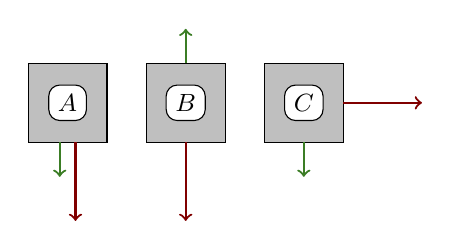
\begin{tikzpicture}[x=10mm,y=10mm, font=\small]

  \begin{scope}[fill=lightgray, draw=black]
    \foreach \x in {0, 1.5, 3}
      \filldraw (\x,0) rectangle  (\x+1,1);
  \end{scope}

  \begin{scope}[every node/.style={fill=white,rectangle, rounded corners, draw=black}]
    \foreach \x/\xtext in {.5/A,2/B,3.5/C}
      \node at (\x,.5) {$\xtext$};
  \end{scope}

  \begin{scope}[thick, ->]
    \begin{scope}[Maroon]
      \draw (.6,0) -- (.6,-1);
      \draw (2,0) -- (2,-1);
      \draw (4,.5) -- (5,.5);
    \end{scope}

    \begin{scope}[OliveGreen]
      \draw (.4,0) -- (.4,-.44);
      \draw (2,1) -- (2,1.44);
      \draw (3.5,0) -- (3.5,-.44);
    \end{scope}
  \end{scope}
\end{tikzpicture}
 \caption{Esercizio \ref{ese:B.18}.}\label{fig:B.16}
\end{minipage}
\end{figure}
\pagebreak

\subsubsection*{\thechapter.6 - Proprietà riflessiva}

\begin{esercizio}
\label{ese:B.19}
Quali relazioni sono riflessive?
\begin{center}
\begin{tabular}{llc}
\toprule
Insieme & Relazione & È riflessiva?\\
\midrule
Numeri naturali & essere divisibile per & \boxSi\quad\boxNo \\
Libri che hai in cartella & avere lo stesso numero di pagine di & \boxSi\quad\boxNo \\
Rette del piano & essere perpendicolare a & \boxSi\quad\boxNo \\
Rette del piano & essere parallela a & \boxSi\quad\boxNo \\
Poligoni & avere lo stesso numero di lati di & \boxSi\quad\boxNo \\
Città della Lombardia & terminare con la stessa vocale & \boxSi\quad\boxNo \\
Parole italiane & essere il plurale di & \boxSi\quad\boxNo \\
\bottomrule
\end{tabular}
\end{center}
\end{esercizio}

\subsubsection*{\thechapter.7 - Proprietà antiriflessiva}

\begin{esercizio}
\label{ese:B.20}
Quali delle seguenti relazioni sono antiriflessive?
\begin{center}
\begin{tabular}{llc}
\toprule
Insieme & Relazione & È antiriflessiva?\\
\midrule
Numeri naturali & essere multiplo di & \boxSi\quad\boxNo \\
Rette del piano & essere perpendicolare a & \boxSi\quad\boxNo \\
Poligoni & avere lo stesso perimetro & \boxSi\quad\boxNo \\
Città del Piemonte & avere più abitanti di & \boxSi\quad\boxNo \\
Parole italiane & essere il femminile di & \boxSi\quad\boxNo \\
Fiumi italiani & essere affluente di & \boxSi\quad\boxNo \\
Persone & essere figlio di & \boxSi\quad\boxNo \\
\bottomrule
\end{tabular}
\end{center}
\end{esercizio}

\subsubsection*{\thechapter.8 - Proprietà simmetrica}

\begin{esercizio}
\label{ese:B.21}
Riconosci le relazioni simmetriche:
\begin{center}
\begin{tabular}{llc}
\toprule
Insieme & Relazione & È simmetrica?\\
\midrule
Città d'Italia & appartenere alla stessa regione & \boxSi\quad\boxNo \\
Rette del piano & essere perpendicolare a & \boxSi\quad\boxNo \\
Solidi & avere lo stesso volume di & \boxSi\quad\boxNo \\
Persone & essere il padre di & \boxSi\quad\boxNo \\
Persone & essere fratello o sorella di & \boxSi\quad\boxNo \\
Numeri naturali & avere lo stesso numero di cifre di & \boxSi\quad\boxNo \\
Fiumi d'Europa & essere affluente di & \boxSi\quad\boxNo \\
Numeri interi & essere il quadrato di & \boxSi\quad\boxNo \\
\bottomrule
\end{tabular}
\end{center}

Le relazioni degli ultimi due casi non godono della proprietà simmetrica. Infatti:
\begin{itemize*}
\item la proposizione ``Il Ticino è un affluente del Po'' è vera, ma non lo è la proposizione che da essa si
ottiene scambiando il soggetto con il complemento;
\item se un numero intero è il quadrato di un altro (ad esempio~$+25$ è il quadrato di~$+5$), non è vero il contrario (infatti~$+5$ non è il quadrato di~$+25$).
\end{itemize*}
\end{esercizio}

\subsubsection*{\thechapter.9 - Proprietà antisimmetrica}

\begin{esercizio}
\label{ese:B.22}
Riconosci le relazioni antisimmetriche:
\begin{center}
\begin{tabular}{llc}
\toprule
Insieme & Relazione & È antisimmetrica?\\
\midrule
Numeri naturali & essere divisibile per & \boxSi\quad\boxNo \\
Rette del piano & essere perpendicolare a & \boxSi\quad\boxNo \\
Poligoni & avere lo stesso perimetro di & \boxSi\quad\boxNo \\
Angoli & essere complementare a & \boxSi\quad\boxNo \\
Città del Lazio & essere nella stessa provincia di & \boxSi\quad\boxNo \\
\bottomrule
\end{tabular}
\end{center}
\end{esercizio}

\subsubsection*{\thechapter.10 - Proprietà transitiva}

\begin{esercizio}
\label{ese:B.23}
Verifica se, nell'insieme ~$\insN$ dei numeri naturali, la relazione~$\Rel$: ``avere lo stesso numero di cifre'' gode della proprietà transitiva.
Completa le proposizioni e rappresenta~$\Rel$ con un grafo:

\begin{enumeratea}
\item da~$18 \,\Rel\,50$ e~$50 \,\Rel\, \ldots$ segue~$\ldots \,\Rel\, \ldots$;
\item da~$\ldots \,\Rel\,555$ e~$\ldots \,\Rel\,267$ segue~$\ldots \,\Rel\, \ldots$
\end{enumeratea}
\end{esercizio}

\begin{esercizio}
\label{ese:B.24}
Indica quale tra le seguenti relazioni è transitiva:
\begin{center}
\begin{tabular}{llc}
\toprule
Insieme & Relazione & È transitiva?\\
\midrule
Numeri naturali & essere multiplo di & \boxSi\quad\boxNo \\
Regioni d'Italia & essere più a nord di & \boxSi\quad\boxNo \\
Numeri interi & essere minore di & \boxSi\quad\boxNo \\
Rette del piano & essere perpendicolare a & \boxSi\quad\boxNo \\
Persone & essere padre di & \boxSi\quad\boxNo \\
Stati d'Europa & confinare con & \boxSi\quad\boxNo \\
\bottomrule
\end{tabular}
\end{center}
\end{esercizio}

\begin{esercizio}
\label{ese:B.25}
Dai una rappresentazione tabulare dell'insieme~$H = \{ x \in \insN \mid  0 \le x \le~12 \}$; determina il resto della divisione di ciascun numero di~$H$ con~4,
compila la tabella come suggerito nell'esempio:
\begin{center}
\begin{tabular}{lccccccccccccc}
\toprule
operazione & $0:4$ & $1:4$ & $2:4$ & & & & & & & & & & $12:4$ \\
resto & 0 & 1 & & & & & & & & & & & 0 \\
\bottomrule
\end{tabular}
\end{center}
Introduciamo in~$H$ la relazione~$x \,\Rel\, y$ se e solo se ``$x$ e~$y$ hanno lo stesso resto nella divisione per~4''.
Costruisci il grafo della relazione e stabilisci se gode della proprietà transitiva.

La stessa relazione~$\Rel$, introdotta nell'insieme dei numeri naturali~$\insN$ è una relazione transitiva?
\end{esercizio}

\begin{multicols}{2}
\begin{esercizio}
\label{ese:B.26}
Completa il grafo in figura~\ref{fig:B.17} a pagina~\pageref{fig:B.17} in modo che la relazione rappresentata diventi transitiva.
\end{esercizio}

\begin{esercizio}
\label{ese:B.27}
Indica la risposta corretta:

\begin{enumeratea}
\TabPositions{12cm}
\item se una relazione è simmetrica, all'insieme~$G_\Rel$ appartengono le coppie del tipo~$(a;b)$ e~$(b;a)$;
\item il grafico cartesiano è un modo per rappresentare una relazione;
\item la matrice di una relazione riflessiva presenta tutti uno sulla diagonale discendente;
\item la matrice di una relazione antiriflessiva non presenta alcun uno sulla diagonale discendente;
\item se una relazione è transitiva, allora è anche simmetrica;
\item se~$(x;y) \in G_\Rel$ e~$(y;z) \in G_\Rel$ qualche volta si ha~$(x;z) \in G_\Rel$;
\item se~$(x;y) \in G_\Rel$ si ha sempre~$(y;x) \in G_\Rel$;
\item una relazione riflessiva presenta nel suo grafo il cappio su ciascun elemento;
\item una relazione binaria è individuata da un predicato che lega due argomenti dell'insieme~$A$;
\item una relazione binaria genera un sottoinsieme del prodotto cartesiano $A \times~A$.
\end{enumeratea}
\end{esercizio}

\begin{esercizio}
\label{ese:B.28}
Con riferimento al grafico cartesiano disegnato nella figura~\ref{fig:B.18}, quale dele seguenti affermazioni è vera?

\begin{enumeratea}
\item nel suo grafo almeno un elemento non presenta il cappio;
\item la relazione è antisimmetrica;
\item la relazione è transitiva;
\item l'insieme~$G_\Rel$ è costituito dalle coppie~$(1;2)$, $(1;4)$, $(3;4)$, $(4;2)$.
\end{enumeratea}
\end{esercizio}
\end{multicols}
\begin{figure}[t]
\begin{minipage}[b]{.45\textwidth}
 \centering
 % (c) 2012 Dimitrios Vrettos - d.vrettos@gmail.com

\begin{tikzpicture}[x=10mm,y=10mm, font=\small, every state/.style={draw=CornflowerBlue, minimum size=0pt}]

\node[state] (X) at (-1,0) {$X$};
\node[state] (H) at (.5,.5) {$H$};
\node[state] (K) at (1,-1) {$K$};
\node[state] (Z) at (-.5,-1) {$Z$};

\begin{scope}[->, Maroon]
\draw (X)--(H);
\draw (X)--(Z);
\draw (H)--(K);
\end{scope}

\end{tikzpicture}

 \caption{Esercizio \ref{ese:B.26}.}\label{fig:B.17}
\end{minipage}\
\begin{minipage}[b]{.45\textwidth}
 \centering
 % (c) 2012 Dimitrios Vrettos - d.vrettos@gmail.com

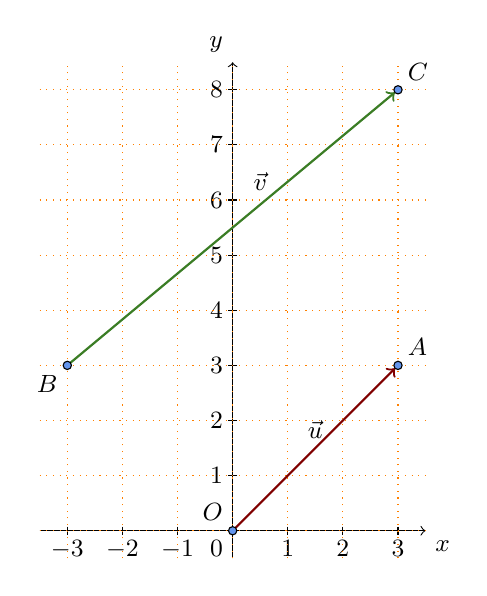
\begin{tikzpicture}[x=7mm,y=7mm, font=\small]

  \begin{scope}[->]
    \draw (-3.5,0) -- (3.5,0) node [below right] {$x$};
    \draw (0,-.5) -- (0,8.5) node[above left] {$y$};
  \end{scope}

  \foreach \x/\xtext in {-3/-3,-2/-2,-1/-1,1/1,2/2,3/3}{
    \node[below] at (\x,0) {$\xtext$};
    \draw (\x,1.5pt) -- (\x,-1.5pt);}
  \foreach \y/\ytext in {1/1,2/2,3/3,4/4,5/5,6/6,7/7,8/8}{
    \node[left] at (0,\y) {$\ytext$};
    \draw (1.5pt,\y) -- (-1.5pt,\y);}
  \node[below left] at (0,0) {$0$};

  \begin{scope}[dotted, orange, step=7mm]
    \draw (-3.5,-.5) grid (3.5,8.5);
  \end{scope}

  \begin{scope}[thick, ->,shorten >=1.5pt]
	\draw[Maroon] (0,0) -- (3,3);  
	\draw[OliveGreen](-3,3) -- (3,8);
      \end{scope}
 

\begin{scope}[fill=CornflowerBlue, draw=black]
\filldraw (0,0) circle (1.5pt)node [above left]{$O$};
\filldraw (3,3) circle (1.5pt)node [above right]{$A$};
\filldraw (-3,3) circle (1.5pt)node [below left]{$B$};
\filldraw (3,8) circle (1.5pt) node [above right]{$C$};
\end{scope}
\node[above] at (1.5,1.5) {$\vec{u}$};
\node[above] at (.5,6) {$\vec{v}$};
\end{tikzpicture}
 \caption{Esercizio \ref{ese:B.28}.}\label{fig:B.18}
\end{minipage}
\end{figure}

\begin{esercizio}
\label{ese:B.29}
Quali proprietà verificano le seguenti relazioni?
\begin{center}
(R = riflessiva, AR = antiriflessiva, S = simmetrica, AS = antisimmetrica, T = transitiva)
\end{center}
\begin{center}
\begin{tabular}{llc}
\toprule
Insieme & Relazione & Proprietà\\
\midrule
Poligoni del piano & avere lo stesso numero di lati & \boxR\quad\boxAR\quad\boxS\quad\boxAS\quad\boxT\\
Numeri naturali & avere lo stesso numero di cifre &\boxR\quad\boxAR\quad\boxS\quad\boxAS\quad\boxT\\
Numeri naturali & essere minore di &\boxR\quad\boxAR\quad\boxS\quad\boxAS\quad\boxT\\
Numeri naturali & essere divisibile per &\boxR\quad\boxAR\quad\boxS\quad\boxAS\quad\boxT\\
$A = \{ x \in \insN \mid  1 \le x \le~5 \}$ & essere multiplo di &\boxR\quad\boxAR\quad\boxS\quad\boxAS\quad\boxT\\
\bottomrule
\end{tabular}
\end{center}
\end{esercizio}

\pagebreak
\subsubsection*{\thechapter.11 - Relazioni di equivalenza}

\begin{esercizio}
\label{ese:B.30}
Quali delle seguenti sono relazioni di equivalenza?
\begin{center}
\begin{tabular}{llc}
\toprule
Relazione & Insieme & È d'equivalenza?\\
\midrule
Essere multiplo & numeri naturali & \boxV\quad\boxF \\
Avere lo stesso numero di sillabe & parole italiane & \boxV\quad\boxF\\
Essere minore & interi relativi & \boxV\quad\boxF \\
Vincere & squadre di calcio & \boxV\quad\boxF\\
Avere lo stesso numero di angoli & poligoni & \boxV\quad\boxF \\
Essere il plurale & parole italiane & \boxV\quad\boxF \\
Essere il cubo & numeri italiani & \boxV\quad\boxF \\
\bottomrule
\end{tabular}
\end{center}
\end{esercizio}
\begin{figure}[t]
 \centering% (c) 2012 Dimitrios Vrettos - d.vrettos@gmail.com

\begin{tikzpicture}[x=10mm,y=10mm, font=\small, every state/.style={draw=CornflowerBlue, minimum size=0pt}, every loop/.style={draw=Maroon}]
\draw (0,0) circle (1.5);
\node at (1.3,1.5) {$A$};
\node at (0,-2) {caso 1};
\node[state] (1) at (-1,0) {$a$};
\node[state] (2) at (.5,.7) {$b$};
\node[state] (3) at (1,0) {$c$};
\node[state] (4) at (-.6,-.7) {$d$};
\node[state] (5) at (.5,-.5) {$e$};
\node[state] (6) at (-.2,.2) {$f$};
\node[state] (7) at (.2,-1.1) {$g$};
\node[state] (8) at (-.4,1.1) {$h$};
\begin{scope}[->]
\path (1) edge[loop above] node{} ()
	(2) edge[loop above] node{} ()
   (6) edge[loop below] node {} ()
(3) edge[loop above] node{} ()
(4) edge[loop left] node{} ()
(7) edge[loop right] node{} ();

\end{scope}
\begin{scope}[-, Maroon]
\draw (1)--(8);
\draw (1)--(6);
\draw (8)--(6);

\draw (2)--(3);
\draw (2)--(5);
\draw (3)--(5);

\draw (4)--(7);
\end{scope}

 \begin{scope}[xshift=32mm]
\draw (0,0) circle (1.5);
\node at (1.3,1.5) {$B$};
\node at (0,-2) {caso 2};
\node[state] (1) at (-1,0) {$a$};
\node[state] (2) at (.5,.7) {$b$};
\node[state] (3) at (1,0) {$c$};
\node[state] (4) at (-.6,-.7) {$d$};
\node[state] (5) at (.5,-.5) {$e$};
\node[state] (6) at (-.2,.2) {$f$};
\node[state] (7) at (.2,-1.1) {$g$};
\node[state] (8) at (-.4,1.1) {$h$};
\begin{scope}[->]
\path (1) edge[loop above] node{} ()
	(2) edge[loop above] node{} ()
   (6) edge[loop below] node {} ()
(3) edge[loop above] node{} ()
(4) edge[loop left] node{} ()
(7) edge[loop right] node{} ()
(5) edge[loop right] node{} ()
(8) edge[loop right] node{} ();

\end{scope}
\begin{scope}[-, Maroon]
\draw (1)--(8);
\draw (1)--(6);
\draw (8)--(6);

\draw (2)--(3);
\draw (2)--(5);
\draw (3)--(5);

\draw (4)--(7);
\end{scope}
 \end{scope}

 \begin{scope}[xshift=64mm]
\draw (0,0) circle (1.5);
\node at (1.3,1.5) {$C$};
\node at (0,-2) {caso 3};
\node[state] (1) at (-1,0) {$a$};
\node[state] (2) at (.5,.7) {$b$};
\node[state] (3) at (1,0) {$c$};
\node[state] (4) at (-.6,-.7) {$d$};
\node[state] (5) at (.5,-.5) {$e$};

\begin{scope}[->]
\path (1) edge[loop above] node{} ()
	(2) edge[loop above] node{} ()
(3) edge[loop above] node{} ()
(4) edge[loop left] node{} ()
(5) edge[loop right] node{} ();

\end{scope}
\begin{scope}[-, Maroon]
\draw (1)--(2);
\draw (2)--(3);
\draw (4)--(5);
\end{scope}
 \end{scope}

 \begin{scope}[xshift=96mm]
\draw (0,0) circle (1.5);
\node at (1.3,1.5) {$D$};
\node at (0,-2) {caso 4};
\node[state] (1) at (-1,0) {$a$};
\node[state] (2) at (.5,.7) {$b$};
\node[state] (3) at (1,0) {$c$};
\node[state] (4) at (-.6,-.7) {$d$};
\node[state] (6) at (.5,-.5) {$f$};
\begin{scope}[->]
\path (1) edge[loop above] node{} ()
	(2) edge[loop above] node{} ()
   (6) edge[loop below] node {} ()
(3) edge[loop above] node{} ()
(4) edge[loop left] node{} ();

\end{scope}
\begin{scope}[->, Maroon]
\draw (3)--(1);
\draw (2)--(1);
\draw (2)--(3);
\end{scope}
 \end{scope}
\end{tikzpicture}
 \caption{Esercizio \ref{ese:B.31}}\label{fig:B.19}
\end{figure}

\begin{multicols}{2}
\begin{esercizio}
\label{ese:B.31}
Analizza i grafi nella figura~\ref{fig:B.19} e individua quello che rappresenta una relazione d'equivalenza:
\begin{itemize*}
\item nel caso~1 non è rappresentata una relazione d'equivalenza perché \dotfill
\item nel caso~2 la presenza del cappio su ciascun elemento indica che la relazione gode della proprietà \ldots,
il fatto che coppie di elementi siano collegate da archi indica che vale la proprietà \ldots, infine terne di elementi godono della proprietà \dotfill

In conclusione\dotfill
\item la relazione del caso~3 non gode della proprietà \dotfill, pertanto \dotfill
\item nel caso~4 sussistono le proprietà \ldots e \ldots, ma non la proprietà \ldots pertanto la relazione \dotfill
\end{itemize*}
\end{esercizio}

\begin{esercizio}
\label{ese:B.32}
Fissa l'attenzione sulla relazione~$\Rel$: ``frequentare la stessa classe'' introdotta nell'insieme~$S$ degli alunni iscritti nella tua scuola.
Verifica che~$\Rel$ è una relazione d'equivalenza. Costruisci le classi d'equivalenza. Quante ne hai potute formare? Come sono indicate nella
realtà che vivi quotidianamente? Determina la partizione~$P(S)$ in classi d'equivalenza e infine l'insieme quoziente~$S/\Rel$.
\end{esercizio}

\begin{esercizio}
\label{ese:B.33}
Studia in~$\insN$ la relazione~$\Rel$: ``avere la stessa cifra delle unità''. Verifica se è una relazione
d'equivalenza, costruisci l'insieme quoziente dopo aver risposto alle seguenti domande:\vspace{-1ex}
\begin{itemize*}
\item quanti numeri naturali sono tra loro equivalenti?
\item da quanti elementi è costituito l'insieme~$\insN/\Rel$?
\item qual è l'elemento che sceglieresti come rappresentante di ciascuna classe?
\end{itemize*}
\end{esercizio}

\begin{esercizio}
\label{ese:B.34}
Considera la relazione~$\Rel$: ``avere lo stesso resto nella divisione per due'' introdotta nell'insieme~$\insN$ e studiane le proprietà.
\begin{itemize*}
\item è una relazione d'equivalenza? Se la risposta è affermativa, costruisci l'insieme quoziente~$\insN/\Rel$.
\item quante classi d'equivalenza hai formato?
\item puoi sfruttare quanto ottenuto per enunciare le definizioni di numero pari e di numero dispari?
\item giustifica, in base allo svolgimento dell'esercizio, l'affermazione: ``L'insieme dei numeri pari è il
complementare in~$\insN$ dell'insieme dei numeri dispari''.
\end{itemize*}
\end{esercizio}

\begin{esercizio}
\label{ese:B.35}
Considera l'insieme~$A = \{x\in\insN \mid  1 \le x \le~20 \}$ e i suoi
sottoinsiemi:~$A_1 =\{$1, 5, 9, 13, 17$\}$, $A_2 =\{$2, 6, 10, 14, 18$\}$, $A_3 =\{$3, 7, 11, 15, 19$\}$, $A_4 =\{$4, 8, 12, 16, 20$\}$.
\begin{enumeratea}
\item Rappresenta gli insiemi con un diagramma di Eulero-Venn;
\item si può affermare che quei sottoinsiemi costituiscono una partizione dell'insieme~$A$?
\item è vero che a ciascuno dei suddetti sottoinsiemi appartengono i numeri di~$A$ aventi lo stesso resto nella divisione per~4?
\item quei sottoinsiemi sono dunque classi d'equivalenza? Qual è il predicato della relazione che le determina?
\end{enumeratea}
\end{esercizio}

\begin{esercizio}
\label{ese:B.36}
Nell'insieme ~$\insN$ dei numeri naturali stabilisci se è d'equivalenza la relazione~$\Rel$: ``$x \,\Rel\, y$ se e solo se~$x$ ha le stesse cifre di~$y$''.
\end{esercizio}

\begin{esercizio}
\label{ese:B.37}
Nell'insieme~$C$ degli alunni della tua classe, verifica se la relazione~$\Rel$: ``$x \,\Rel\, y$ se e solo se il cognome di~$x$ ha la stessa lettera iniziale del
cognome di~$y$'' è d'equivalenza; determina in caso affermativo la partizione dell'insieme~$C$ e l'insieme quoziente~$C/\Rel$.
\end{esercizio}

\begin{esercizio}
\label{ese:B.38}
Nell'insieme delle parole della lingua italiana verifica se la relazione ``$x \,\Rel\, y$ se e solo se~$x$ ha lo stesso numero di lettere di~$y$'' è
una relazione di equivalenza. In caso affermativo individua alcune classi di
equivalenza.
\end{esercizio}

\begin{esercizio}
\label{ese:B.39}
Nell'insieme dei nomi dei giorni della settimana considera la relazione ``$x \,\Rel\, y$ se e solo se~$x$ e~$y$ hanno almeno tre lettere in comune''.
Verifica se è una relazione di equivalenza e in caso affermativo individua le
classi di equivalenza.
\end{esercizio}

\begin{esercizio}
\label{ese:B.40}
Nell'insieme dei numeri naturali da~1 a~100, verifica se la relazione ``$x \,\Rel\, y$ se e solo se~$x$ e~$y$ hanno lo stesso numero di lettere''
è una relazione di equivalenza. Individua quante sono le classi di equivalenza.
Scrivi tutti gli elementi delle classi di equivalenza~$[1]$ e~$[10]$.
\end{esercizio}

\begin{esercizio}
\label{ese:B.41}
Nell'insieme dei numeri naturali da~1 a~100, verifica se la relazione ``$x \,\Rel\, y$ se e solo se~$x+y$ è
dispari'' è una relazione di equivalenza.
\end{esercizio}

\begin{esercizio}
\label{ese:B.42}
Nell'insieme dei nomi dei mesi dell'anno verifica se la relazione ``$x \,\Rel\, y$ se e solo se~$x$ e~$y$ hanno almeno~3 lettere in comune''
è una relazione di equivalenza. Eventualmente individua le classi di equivalenza.
\end{esercizio}

\begin{esercizio}
\label{ese:B.43}
Sia~$S$ un insieme non vuoto in cui è definita una relazione~$\Rel$ riflessiva e transitiva; in~$S$ si definisca la relazione~$\sharp$ ponendo,
per ogni~$x$, $y$ appartenenti a~$X$, $x \,\sharp\, y$ se e solo se~$x \,\Rel\, y$ e~$y \,\Rel\, x$. Verificare che~$\sharp$ è una relazione di equivalenza in~$X$.
\end{esercizio}
\end{multicols}

\begin{figure}[t]
\begin{minipage}[b]{.45\textwidth}
 \centering
 % (c) 2012 Dimitrios Vrettos - d.vrettos@gmail.com

\begin{tikzpicture}[x=10mm,y=10mm, font=\small, every state/.style={draw=CornflowerBlue, minimum size=0pt}, every loop/.style={draw=Maroon}]
\draw (0,0) circle (1.5);
\node at (1.5,1.5) {$T$};
\node[state] (1) at (-.6,.7) {$M$};
\node[state] (2) at (1,.5) {$Z$};
\node[state] (3) at (1,-.5) {$W$};
\node[state] (4) at (-.8,-.7) {$J$};
\node[state] (5) at (0.1,-1.1) {$P$};

\begin{scope}[->, Maroon]
 \draw (1)--(3);
 \draw (1)--(2);
 \draw (2)--(3); 
 \draw (2)--(5); 
 \draw (2)--(4); 
 \draw (3)--(4);
 \draw (5)--(4);
 \draw (5)--(3);
 \draw (1)--(4);
 \draw (1)--(5);
\end{scope}

\end{tikzpicture}

 \caption{Esercizio \ref{ese:B.45}.}\label{fig:B.20}
\end{minipage}\
\begin{minipage}[b]{.45\textwidth}
 \centering
 % (c) 2012 Dimitrios Vrettos - d.vrettos@gmail.com

\begin{tikzpicture}[x=10mm,y=10mm, font=\small]
 \tkzDefPoint(0,0){A}
 \tkzDefShiftPoint[A](30:4.67){C}
 \tkzDefShiftPoint[A](0:5.97){B}

 \tkzMarkAngle[fill=LimeGreen, draw=black, size=.4](B,A,C)
 \tkzMarkAngle[fill=LimeGreen, draw=black, size=.4](C,B,A)

\tkzDrawLine[add=0 and 0, thin,dashed](A,B)
\tkzDrawLine[add=0 and 0, thin](A,C)
\tkzDrawLine[add=0 and 0, thin](B,C)

 \tkzLabelPoints[below](A,B)
\tkzLabelAngle[](B,A,C){$30^\circ$}
\tkzLabelAngle[](C,B,A){$50^\circ$}
 \tkzDrawPoints[color=CornflowerBlue](A,B,C)
 
\end{tikzpicture}
 \caption{Esercizio \ref{ese:B.47}.}\label{fig:B.21}
\end{minipage}
\end{figure}

\begin{multicols}{2}
\subsubsection*{B.12 - Relazioni di ordine}
\begin{esercizio}
\label{ese:B.44}
Nell'insieme~$M =\{$1, 8, 3, 4, 10, 2, 7, 0, 5, 9, 6$\}$ viene introdotta la relazione~$\Rel$ così definita: ``$x \,\Rel\, y$ se e solo se~$y-x$ appartiene a ~$\insN$''.
La relazione è riflessiva? La relazione è antisimmetrica? La relazione è transitiva? \`E vero che due elementi
distinti sono sempre confrontabili?
\end{esercizio}

\begin{esercizio}
\label{ese:B.45}
\`E assegnata la relazione~$R$ nell'insieme~$T$, rappresentata col grafo di figura~\ref{fig:B.20}.
Analizzando il grafo, rispondi alle domande:
\begin{itemize*}
\item la relazione è riflessiva?
\item la relazione è antisimmetrica?
\item la relazione è transitiva?
\item due elementi distinti sono sempre confrontabili?
\end{itemize*}
Alla prima domanda avrai risposto negativamente: nessun elemento dell'insieme~$T$ è in relazione con se stesso, mentre valgono le proprietà antisimmetrica e transitiva.
Infine scelti due elementi qualsiasi dell'insieme~$T$, essi sono sempre confrontabili.
\end{esercizio}

\begin{esercizio}
\label{ese:B.46}
Verifica che la relazione~$\Rel$: ``essere divisore'' introdotta nell'insieme~$J =\{$3, 6, 10, 15, 21$\}$ è una relazione d'ordine parziale in senso largo.
\end{esercizio}

\begin{esercizio}
\label{ese:B.47}
Perché la relazione~$\Rel$ rappresentata dal grafico cartesiano riportato nella figura~\ref{fig:B.21}, pur essendo una relazione d'ordine non può essere
classificata in nessuna delle tipologie studiate? Dai una breve motivazione indicando quali proprietà non sono soddisfatte dalla relazione rappresentata.
\end{esercizio}

\begin{esercizio}
\label{ese:B.48}
Nell'insieme degli studenti della tua classe determina le proprietà della relazione~$\Rel$: ``$x \,\Rel\, y$ se e solo se l'altezza di~$x$ non supera l'altezza di~$y$''. \`E una relazione d'ordine? Di quale tipo?
\end{esercizio}

\begin{esercizio}
\label{ese:B.49}
Nell'insieme~$A = \{$12, 4, 2, 8, 3, 21, 5, 60$\}$ la relazione~$\Rel$: ``essere divisibile'' è una relazione d'ordine? Se lo è, di che tipo di relazione si tratta? Totale, parziale, in senso largo, in senso stretto?
\end{esercizio}

\begin{esercizio}
\label{ese:B.50}
Nell'insieme ~$\insN - \{ 0 \}$ la relazione ``essere divisibile'' è d'ordine totale in senso largo?
\end{esercizio}

\begin{esercizio}
\label{ese:B.51}
Rappresenta nelle tre modalità studiate una relazione che sia solo simmetrica; ripeti le rappresentazioni per una relazione che sia almeno simmetrica. Quale significato hanno le due richieste formulate sopra?
\end{esercizio}

\begin{esercizio}
\label{ese:B.52}
L'insieme~$G_\Rel$ di una relazione introdotta nell'insieme~$A = \{a$, $b$, $c$, $d$, $e\}$ è~$G_\Rel = \{ (a;a)$, $(a;b)$, $(b;b)$, $(d;d)$, $(c;d)$, $(d;e)$, $(e;e)\}$.
Quale delle seguenti affermazioni è vera
\begin{enumeratea}
\item $\Rel$ è una relazione antiriflessiva;
\item $\Rel$ è una relazione solo antisimmetrica;
\item $\Rel$ è una relazione riflessiva;
\item $\Rel$ è una relazione transitiva e antisimmetrica;
\end{enumeratea}
\end{esercizio}

\begin{esercizio}
\label{ese:B.53}
La relazione~$\Rel$: ``essere vicini di banco'' inserita nell'insieme degli alunni della tua classe è una
relazione d'equivalenza? \`E una relazione d'ordine?
\end{esercizio}

\end{multicols}

\begin{figure}[t]
\begin{minipage}[b]{1\textwidth}
 \centering
 % (c) 2012 Dimitrios Vrettos - d.vrettos@gmail.com

\begin{tikzpicture}[x=10mm,y=10mm, font=\small, every state/.style={draw=CornflowerBlue, minimum size=0pt}, every loop/.style={draw=Maroon}]
\draw (0,0) circle (1.5);
\node at (0,-2) {1};
\node[state] (1) at (-.6,.7) {$-12$};
\node[state] (2) at (.5,.5) {$-1$};
\node[state] (3) at (.5,-.8) {$-15$};
\node[state] (4) at (-.6,-.7) {$-7$};

\begin{scope}[->, Maroon]
 \draw (3)--(1);
 \draw (1)--(2);
 \draw (3)--(2); 
 \draw (3)--(4);
\draw (4)--(2);
 \draw (1)--(4);
\end{scope}

 \begin{scope}[xshift=31mm]
\draw (0,0) circle (1.5);
\node at (0,-2) {2};
\node[state] (1) at (-1,0) {$a$};
\node[state] (2) at (.5,.7) {$b$};
\node[state] (3) at (.5,-.5) {$c$};
\node[state] (4) at (-.6,-.7) {$m$};

\begin{scope}[->]
\path (1) edge[loop above] node{} ()
	(2) edge[loop above] node{} ()
(3) edge[loop below] node{} ()
(4) edge[loop left] node{} ();

\end{scope}
\begin{scope}[->, Maroon]
\draw (1)--(3);
\draw (1)--(2);
\draw (2)--(3);
\end{scope}
 \end{scope}

 \begin{scope}[xshift=62mm]
\draw (0,0) circle (1.5);
\node at (0,-2) {3};
\node[state] (1) at (-1,0) {$M$};
\node[state] (2) at (0,.8) {$B$};
\node[state] (3) at (1,0) {$C$};
\node[state] (4) at (0,-1) {$F$};


\begin{scope}[->]
\path (1) edge[loop above] node{} ()
	(2) edge[loop above] node{} ()
(3) edge[loop above] node{} ()
(4) edge[loop left] node{} ();

\end{scope}
\begin{scope}[->, Maroon]
\draw (1)--(2);
\draw (1)--(3);
\draw (1)--(4);
\draw (2)--(4);
\draw (4)--(3);
\end{scope}
 \end{scope}
\end{tikzpicture}
 \caption{Esercizio \ref{ese:B.58}.}\label{fig:B.22}
\end{minipage}
\hfill
\begin{minipage}[b]{\textwidth}
 \centering
 % (c) 2012 Dimitrios Vrettos - d.vrettos@gmail.com

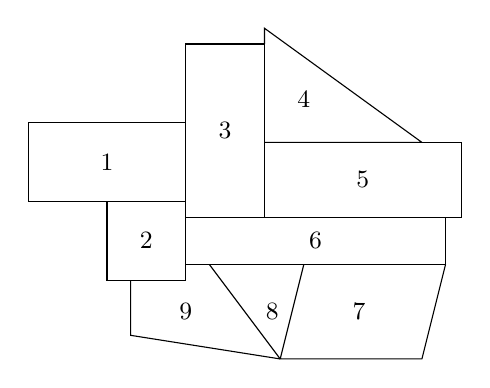
\begin{tikzpicture}[x=10mm,y=10mm, font=\small]
\draw (0,0) rectangle  (2,1) node[midway] {1};
\draw (1,-1) rectangle  (2,0) node[midway] {2};
\draw (2,-.2) rectangle  (3,2) node[midway] {3};
\draw (3,2)-- (3,2.2) -- (5,.75) --(3,.75);
\draw (3,.75) rectangle  (5.5,-.2) node[midway] {5};
\draw (2,-.2) rectangle  (5.3,-.8) node[midway] {6};
\draw (5.3,-.8) -- (5,-2) --(3.2,-2) --(3.5,-.8);
\draw (3.2,-2) -- (2.3,-.8);
\draw (3.2,-2) -- (1.3,-1.7)-- (1.3,-1);
 \node at (3.5,1.3) {4};
 \node at (4.2,-1.4) {7};
 \node at (3.1,-1.4) {8};
 \node at (2,-1.4) {9};
\end{tikzpicture}
 \caption{Esercizio \ref{ese:B.62}.}\label{fig:B.23}
\end{minipage}
\end{figure}

\begin{multicols}{2}

\begin{esercizio}
\label{ese:B.54}
I tre sottoinsiemi~$A_1 = \{$36, 135, 432$\}$, $A_2 = \{65\}$ e $A_3 = \{$66, $3\,522$, 93, 435$\}$ dell'insieme~$A = \{$36, 65, 66, 93, 135, 432, 435, $3\,522\}$ costituiscono una partizione dell'insieme~$A$? Sapresti trovare una caratteristica per gli elementi di ciascun sottoinsieme? $A_1$, $A_2$, $A_3$ sono classi d'equivalenza?
\end{esercizio}

\begin{esercizio}
\label{ese:B.55}
Nell'insieme ~$\insN$ la relazione~$\Rel$: ``$x \,\Rel\, y$ se e solo se~$x \cdot y$ è un numero dispari'' è d'equivalenza?
\end{esercizio}

\begin{esercizio}
\label{ese:B.56}
La relazione~$\Rel$: ``$x \,\Rel\, y$ se e solo se~$x$ sta nella stessa nazione di~$y$'' nell'insieme~$K= \{$Parigi, Madrid, Milano, Siviglia, Bari, Granada, Venezia, Lione$\}$
è d'equivalenza? Costruisci~$A/\Rel$.
\end{esercizio}

\begin{esercizio}
\label{ese:B.57}
Verifica se la relazione~$\Rel$ assegnata con la matrice rappresentata
sotto è d'equivalenza. In caso positivo determina la partizione dell'insieme~$A =\{\square, \lozenge, \infty, \nabla\}$ e l'insieme
quoziente~$A/\Rel$.

\begin{center}
\begin{tabular}{ccccc}
\toprule
 & $\square$ & $\lozenge$ & $\infty$ & $\nabla$\\
\midrule
 $\square$ & 1 & 1 & 0 & 0 \\
 $\lozenge$ & 1 & 1 & 0 & 0 \\
 $\infty$ & 0 & 0 & 1 & 1\\
 $\nabla$ & 0 & 0 & 1 & 1\\
\bottomrule
\end{tabular}
\end{center}
\end{esercizio}

\begin{esercizio}
\label{ese:B.58}
In un torneo di pallavolo gareggiano quattro squadre A, B, C, D; rappresenta con un grafo a frecce le seguenti informazioni, relative alle prime tre giornate:
\begin{itemize*}
\item 1\textsuperscript{a} giornata: A vince contro B; C vince contro D;
\item 2\textsuperscript{a} giornata: D vince contro A; B vince contro C;
\item 3\textsuperscript{a} giornata: A vince contro C; B vince contro D;
\end{itemize*}
Il~4\textsuperscript{o} giorno si gioca la semifinale tra le prime due classificate e le altre due. Se per ogni vittoria si ottiene un punteggio di~10 punti e per ogni sconfitta un punteggio
di~2 punti, quale squadra gioca la semifinale con B?
Il torneo è vinto dalla squadra C. Rappresenta con un grafo a frecce la situazione della semifinale e quella
della finale. \`E unica la risposta a quest'ultimo quesito?
\end{esercizio}

\begin{esercizio}
\label{ese:B.59}
Associa a ciascun grafo della figura~\ref{fig:B.22} a pagina~\pageref{fig:B.22} la corretta relazione d'ordine:
\begin{enumeratea}
\item ordine totale in senso largo;
\item ordine totale in senso stretto;
\item ordine parziale in senso largo;
\item ordine parziale in senso stretto.
\end{enumeratea}
\end{esercizio}

\begin{esercizio}
\label{ese:B.60}
Nell'insieme di tutti gli iscritti a Facebook, determina le proprietà della relazione~$\Rel$: ``$x \,\Rel\, y$ se e solo se il numero di amici di~$x$ supera
il numero di amici di~$y$''. \`E una relazione d'ordine? Se sì, di quale tipo?
\end{esercizio}

\begin{esercizio}
\label{ese:B.61}
Nell'insieme delle parole della lingua italiana, verifica se la relazione ``$x \,\Rel\, y$ se e solo se~$x$ ha più lettere di~$y$'' è una relazione d'ordine.
In caso affermativo dire se è totale o parziale, in senso largo o in senso stretto.
\end{esercizio}

\begin{esercizio}
\label{ese:B.62}
Nell'insieme dei numeri naturali, verifica se la relazione ``$x \,\Rel\, y$ se e solo se~$x$ ha un numero di cifre maggiore del numero di cifre di~$y$''
è una relazione d'ordine. In caso affermativo dire se è totale o parziale, in senso largo o in senso stretto.
\end{esercizio}

\begin{esercizio}
\label{ese:B.63}
Andrea, insegnante di grafica, ha chiesto ai suoi alunni di usare il minimo numero di colori per colorare il modello della figura~\ref{fig:B.23} a pagina~\pageref{fig:B.23},
in modo che poligoni confinanti non risultino con lo stesso colore. Come si può risolvere il problema? [Risposta: 3 colori]

\emph{Traccia di soluzione}: Nell'insieme~$Z =\{$1, 2, 3, 4, 5, 6, 7, 8, 9$\}$ studia la relazione~$\Rel$: ``confinare con'', rappresentandola con un grafico cartesiano e sfrutta
i risultati trovati per risolvere il problema.
La soluzione può essere trovata fissando un punto interno a ciascuna regione: due punti sono uniti se e solo se le regioni confinano, il segmento che li congiunge
deve attraversare solo il loro confine comune; i punti che non sono congiunti indicano regioni che avranno lo stesso colore.
\end{esercizio}
\end{multicols}

\cleardoublepage
